\documentclass[
		fontsize=12pt,		% Schriftgröße 12pt
		toc=listof,		% Schreibt Tabellen/Abbildungs-Verzeichnisse auch mit ins Inhaltsverzeichnis
		%toc=bib,		% Literaturverzeichnis im Inhaltsverzeichnis aufführen
		%bibliography=openstyle	% Literaturverzeichnis etwas auflockern
		headsepline,		% Linie unter Kolumnentitel
		twoside=false,		% Layout für einseitigen Druck
		BCOR=12mm,		% Bindekorrektur: bei Buch normalerweise 12mm
		DIV=14,			% DIV-Wert fuer die Erstellung des Satzspiegels, siehe scrguide
		parskip=false,		% Absatzeinzug (Standard), half: kein Einzug, Halber Zeilenabstand, ...
		captions=tableheading,	% korrekte Abstände bei Tabellenüberschriften
		draft=false,		% true: Kennzeichnung von Absätzen, die manuell bearbeitet werden müssen, false: aus
		paper=A4,		% A4 Seite
		pagesize=automedia,	% Setzen der korrektern Papiergröße für Ausgabemedien
		numbers=noendperiod	% Auch wenn \appendix genutzt wird, keine Punkte hinter der Nummerierung (Regel im Duden sieht allerdings Punkt vor)
	]{scrbook}			% aus Komascript für Bücher
%%%%%%%%%%%%%%%%%%%%%%%%%%%%%%%%%%%%%%%%%%%%%%%%%%%%%%%%%%%%%%%%%%%%%%%%%%%%%%%%


% Pakete
\usepackage{cmap}		% to make the PDF files "searchable and copyable" in pdf viewer
\usepackage[ngerman]{babel}	% deutschsprachig
\usepackage[utf8]{inputenc}	% utf8 encoding
\usepackage[T1]{fontenc}	% Schriftkodierung
\usepackage{lmodern}		% skalierbare Schriftfamilie "Latin Modern" (default: bitmapped "Computer Modern")
\usepackage{graphicx}		% Einbinden von Grafiken
\usepackage{booktabs}		% weitere Linien zur Strukturierung von Tabellen (\toprule, ...)
\usepackage{multirow}		% mehrere Zeilen in einer Tabelle zusammenfassen
\usepackage{ltxtable}		% longtable und tabularx vereint in einer Tabelle, lädt automatisch beide Pakete
\usepackage{rotating}		% Text drehen
\usepackage{amsmath}		% Matheumgebung
\usepackage{amssymb}		% Zusatzsymbole zB Square Vartriangle etc
\usepackage{moreverb}		% erweiterte verbatim Umgebung
\usepackage{listings}		% Listings -> Quellcodedarstellung für viele verschiedene Sprachen
\usepackage{subfigure}		% Unterbilder
\usepackage{xcolor}		% Farbdefinitionen möglich
\usepackage{pdfpages}		% Einbinden von PDF Seiten aus PDF Dokument
\usepackage{nicefrac}		% Darstellung eines Bruchs im Fließtext; Aussehen zB 1/4
\usepackage{acronym}		% Abkürzungsverzeichnis --> nur verwendete Abkürzungen listen [printonlyused]
%\usepackage{bibgerm}		% deutsches Literaturverzeichnis
\usepackage{caption}		% viele caption Formatierungsmöglichkeiten
\usepackage{setspace}		% Zeilenabstand festlegen
\usepackage{microtype}		% Verbessert Textsatz
\usepackage{fixltx2e}		% Verbessert einige Kernkompetenzen von LaTeX2e
\usepackage{ellipsis}		% Korrigiert den Weißraum um Auslassungspunkte
\usepackage{units}		% Einheiten komfortabel darstellen \unit[Zahlenwert]{Einheit}
\usepackage{textcomp}		% einige Text-Mode Mathe Symbole, wie zB Mal-Zeichen x (siehe The Comprehensive LaTeX Symbol List)
\usepackage{gensymb}		% celsius, micro, ohm, perthousand, degree in Mathe und Textmodus
%%%%%%%%%%%%%%%%%%%%%%%%%%%%%%%%%%%%%%%%%%%%%%%%%%%%%%%%%%%%%%%%%%%%%%%%%%%%%%%%

% Einbindung von allen Grafikformaten möglich
\usepackage{pst-pdf} % pstricks und ps grafiken in pdflatex
\usepackage{pst-all}
\usepackage{pstricks-add}
%%%%%%%%%%%%%%%%%%%%%%%%%%%%%%%%%%%%%%%%%%%%%%%%%%%%%%%%%%%%%%%%%%%%%%%%%%%%%%%%


% für Fließumgebungen
% Platzierung H zwingt LaTeX Fließumgebungen genau an diese Stelle zu setzen
\usepackage{float}
\usepackage{wrapfig}
%%%%%%%%%%%%%%%%%%%%%%%%%%%%%%%%%%%%%%%%%%%%%%%%%%%%%%%%%%%%%%%%%%%%%%%%%%%%%%%%


% Kopf- und Fußzeilen
\usepackage[headsepline]{scrpage2}	% Paket, Linie unter Kopfangabe
\clearscrheadfoot			% löscht alle bisherigen Kopf- und Fußzeilen
\pagestyle{scrheadings}			% selbstgebastelte Kopf-/Fußzeilen
\automark{chapter}			% \automark[<rechte seite>]{<linke seite>}
\chead[Multicast Test Tool - System Architecture Specification - Team 1]{Multicast Test Tool - System Architecture Specification - Team 1} 
\cfoot[-\,\pagemark\,-]{-\,\pagemark\,-}% setzt Fußzeile [] -> chapterseiten; {} -> alle anderen Seiten
%%%%%%%%%%%%%%%%%%%%%%%%%%%%%%%%%%%%%%%%%%%%%%%%%%%%%%%%%%%%%%%%%%%%%%%%%%%%%%%%



% Schusterjungen und Hurenkinder vermeiden
\clubpenalty = 10000
\widowpenalty = 10000
\displaywidowpenalty = 10000
%%%%%%%%%%%%%%%%%%%%%%%%%%%%%%%%%%%%%%%%%%%%%%%%%%%%%%%%%%%%%%%%%%%%%%%%%%%%%%%%



% Farbdefinitionen
\definecolor{fill}{rgb}{1,1,0.73}
%%%%%%%%%%%%%%%%%%%%%%%%%%%%%%%%%%%%%%%%%%%%%%%%%%%%%%%%%%%%%%%%%%%%%%%%%%%%%%%%




% Workaround eines Bugs des wrapfig Paketes
% Entfernen wenn neue Version den Pakets verfügbar ist
% wenn ein umflossenes Bild nicht vollständig umflossen wird
% muss der Absatz geschlossen werden: dazu dann den Befehl
% \wrapfill hinter dem Absatz notieren
\usepackage{blindtext,wrapfig}
\makeatletter
\newcommand\wrapfill{\par
    \ifx\parshape\WF@fudgeparshape
    \nobreak
    \vskip-\baselineskip
    \vskip\c@WF@wrappedlines\baselineskip
    \allowbreak
    \WFclear
    \fi
}
\makeatother
%%%%%%%%%%%%%%%%%%%%%%%%%%%%%%%%%%%%%%%%%%%%%%%



% interne und externe Links werden als Hyperlinks übersetzt
% viele andere Optionen für pdf viewer möglich
% pdf metadaten
\usepackage{hyperref}
\hypersetup{pdftitle={SAS},
	pdfauthor={Team 1},
	pdfsubject={SAS - System Architecture Specification},
	pdfcreator={LaTeX (TexLive 2008)},
	pdfproducer={LaTeX (TexLive 2008)},
	pdfkeywords={},
	colorlinks=true,
	urlcolor=black,
	linkcolor=black,
	citecolor=black,
	unicode=true
}
%%%%%%%%%%%%%%%%%%%%%%%%%%%%%%%%%%%%%%%%%%%%%%%%%%%%%%%%%%%%%%%%%%%%%%%%%%%%%%%%


% caption setup
% hang: bereich unter dem bezeichner bleibt frei;
% figurename: Bezeichner umdefinieren;
% margin: Einzug links und rechts
\captionsetup{format=hang,margin=30pt}
\captionsetup[lstlisting]{skip=13pt}
%%%%%%%%%%%%%%%%%%%%%%%%%%%%%%%%%%%%%%%%%%%%%%%%%%%%%%%%%%%%%%%%%%%%%%%%%%%%%%%%



%% Listings-Formatierung
\lstset{%
	language=Java, %
	basicstyle=\tiny,%\scriptsize,
	frame=trbl,%
	numbers=left,%
	breaklines=true,
	prebreak=\mbox{$\hookleftarrow$},
	postbreak=\mbox{$\longrightarrow$},
	breakatwhitespace=true,
	captionpos=t,%
	showstringspaces=false,
	numberstyle=\tiny,%
	commentstyle=\color{red},%
	keywordstyle=\bfseries\color{blue},%
	backgroundcolor=\color{fill},%
	rulecolor=\color{gray}%
}
%%%%%%%%%%%%%%%%%%%%%%%%%%%%%%%%%%%%%%%%%%%%%%%%%%%%%%%%%%%%%%%%%%%%%%%%%%%%%%%%

\setcounter{secnumdepth}{2}
\setcounter{tocdepth}{1}

% Tabellen
% neuer Spaltentyp C --> zentrierte X Spalten
\newcolumntype{C}{>{\centering\arraybackslash}X}
% Größere Höhe von Tabellenzellen
\renewcommand{\arraystretch}{1.3}
%%%%%%%%%%%%%%%%%%%%%%%%%%%%%%%%%%%%%%%%%%%%%%%%%%%%%%%%%%%%%%%%%%%%%%%%%%%%%%%%



% chapterüberschriften ohne Abstand zum Kopf festlegen
% \renewcommand*{\chapterheadstartvskip}{\vspace*{-\topskip}}
%%%%%%%%%%%%%%%%%%%%%%%%%%%%%%%%%%%%%%%%%%%%%%%%%%%%%%%%%%%%%%%%%%%%%%%%%%%%%%%%



% 1,5-Zeilenabstand (Paket setspace erforderlich)
\onehalfspacing
% Neuberechnung des Satzspiegels für neuen Zeilenabstand (DIV Angabe aus der
% Klassendeklartion übernommen)
\KOMAoptions{DIV=last}
%%%%%%%%%%%%%%%%%%%%%%%%%%%%%%%%%%%%%%%%%%%%%%%%%%%%%%%%%%%%%%%%%%%%%%%%%%%%%%%%



% Befehle für Hoch und Tiefstellen innerhalb eines Textes
\newcommand{\up}[2]{#1\textsuperscript{#2}}
\newcommand{\down}[2]{#1\textsubscript{#2}}
%%%%%%%%%%%%%%%%%%%%%%%%%%%%%%%%%%%%%%%%%%%%%%%%%%%%%%%%%%%%%%%%%%%%%%%%%%%%%%%%



% Beginn des Dokuments
\begin{document}

	%Vorspann
	\frontmatter

	% große römische Ziffern für die Seitennummern im Vorspann (Standard sind kleine römische Ziffern)
	\pagenumbering{Roman}

	% Includes Vorspann
	% Titelseite
	%%%%%%%%%%%%%%%%%%%%%%%%%%%%%%%%%%%%%%%%%%%%%%%%%%%%%%%%%%%%%%
% \titlehead	Kopfzeile der Titelseite
% \subject	Thema des Dokumentes
% \title	Titel des Dokumentes
% \subtitle	Untertitel
% \author	Autor des Dokumentes
% \date	Datum der Veröffentlichung
% \dedication	Widmung ;-)
% \publishers	Herausgeber
% \thanks	Fußnote
% \begin{abstract}
%   ...
% \end{abstract}

\newcommand{\mytitle}{}
\newcommand{\setmytitle}[1]{\renewcommand{\mytitle}{#1}}

\newcommand{\myauthor}{}
\newcommand{\setmyauthor}[1]{\renewcommand{\myauthor}{#1}}

\newcommand{\mysubject}{}
\newcommand{\setmysubject}[1]{\renewcommand{\mysubject}{#1}}

\setmytitle{"`Multicast Test Tool"'}
\setmyauthor{Tobias Stöckel, Tobias Schoknecht}
\setmysubject{Moduldokumentation GUI-Design}

\titlehead{%
	\fontsize{14pt}{12} \selectfont%
	\textbf{Fakultät:} \\%
	\\%
	
\includegraphics[width=5cm]{images/dhbw.jpg}

}

\title{}
\subject{\vspace{0.1cm}%
	\mysubject \\
	\vspace{0.5cm}%
	\mytitle%
	\vspace{-1.5cm}%
}
\author{%
	{
	\renewcommand{\arraystretch}{1}
	\fontsize{12pt}{12} \selectfont%
	\begin{tabular}{lcl}%
		Vorgelegt von & : & Team 1 \\%
		Verantwortlicher & : & Tobias Stöckel \\%
		Priorität aus Auftraggebersicht & : & mittel\\
		Priorität aus Auftragnehmersicht & : & hoch\\
		Stabilität & : & fest\\
		Kritikalität & : & niedrig\\
		Entwicklungsrisiko & : & niedrig\\
		Kategorie & : & Internes Dokument\\
		Version & : & 1.0\\
	 \end{tabular}%
	}
}
\date{

\includegraphics[height=3cm]{images/Logo.jpg}\\
16.05.2011
}

%%%%%%%%%%%%%%%%%%%%%%%%%%%%%%%%%%%%%%%%%%%%%%%%%%%%%%%%%%%%%%%%
\maketitle
	% Includes Verantwortliche
	% Titelseite
	\chapter*{Projektteam}
\textbf{Produkt Manager}\\
Tobias St"ockel\\
\newline
\textbf{Projekt Leiter}\\
David Hildenbrand\\
\newline
\textbf{Leitende Ingenieure}\\
Jeffrey Jedele\\
Konstantin Weitz\\
\newline
\textbf{Technische Dokumentation}\\
Tobias Schoknecht\\
\newline\textbf{Systemtest}\\
Ramin Safarpour\\
\newline
	%%%%%%%%%%%%%%%%%%%%%%%%%%%%%%%%%%%%%%%%%%%%%%%%%%%%%%%%%%%%%%%%%%%%%%%%%%%%%%%%
	% offizielle Aufgabenstellung
%	\include{./chapter/aufgabenstellung}
	%%%%%%%%%%%%%%%%%%%%%%%%%%%%%%%%%%%%%%%%%%%%%%%%%%%%%%%%%%%%%%%%%%%%%%%%%%%%%%%%
	% Selbstständigkeitserklärung
	%\include{./chapter/declaration_of_primary_authorship}
	%%%%%%%%%%%%%%%%%%%%%%%%%%%%%%%%%%%%%%%%%%%%%%%%%%%%%%%%%%%%%%%%%%%%%%%%%%%%%%%%
	% Inhaltsverzeichnis
	\tableofcontents
	%%%%%%%%%%%%%%%%%%%%%%%%%%%%%%%%%%%%%%%%%%%%%%%%%%%%%%%%%%%%%%%%%%%%%%%%%%%%%%%%
	% Abbildungsverzeichnis
	\listoffigures
	%%%%%%%%%%%%%%%%%%%%%%%%%%%%%%%%%%%%%%%%%%%%%%%%%%%%%%%%%%%%%%%%%%%%%%%%%%%%%%%%
	% Tabellenverzeichnis
	\listoftables
	%%%%%%%%%%%%%%%%%%%%%%%%%%%%%%%%%%%%%%%%%%%%%%%%%%%%%%%%%%%%%%%%%%%%%%%%%%%%%%%%
	% Listings-Verzeichnis
%	\renewcommand{\lstlistlistingname}{Quelltexte}
%	\lstlistoflistings
	%%%%%%%%%%%%%%%%%%%%%%%%%%%%%%%%%%%%%%%%%%%%%%%%%%%%%%%%%%%%%%%%%%%%%%%%%%%%%%%%
	% Abkürzungsverzeichnis/Formelzeichen
	%\addcontentsline{toc}{chapter}{Abkürzungsverzeichnis}
\chapter*{Abkürzungsverzeichnis}

    \begin{description}
        \item[PPS] Packets Per Second. (Multicast-) Pakete pro Sekunde. Einheit
        für Datensende- und empfangsrate.
    \end{description}
	%%%%%%%%%%%%%%%%%%%%%%%%%%%%%%%%%%%%%%%%%%%%%%%%%%%%%%%%%%%%%%%%%%%%%%%%%%%%%%%%
	%%%%%%%%%%%%%%%%%%%%%%%%%%%%%%%%%%%%%%%%%%%%%%%%%%%%%%%%%%%%%%%%%%%%%%%%%%%%%%%%

	% Hauptteil
	\mainmatter

	\chapter{Einführung und Zielsetzung}
	\label{chap:1}
	% This documents structure is based on a template from the following website
% http://www.arc42.de/

\section{Aufgabenstellung}
\label{sec:1:aufg}


Da die Multicast-Fähigkeit nur optional im weit verbeiteten IP-Standard
verankert ist, wird sie von vielen Hard- und Softwarekomponenten nicht richtig
implementiert.\\
Das Multicast-Test-Tool wird es ermöglichen, die Multicasting-Fähigkeiten eines
Netzwerks über IPv4 und IPv6 hinsichtlich Funktionalität, Synchronizität und
Traversierungsdauer auf einen Blick mess- und verifizierbar zu machen.\\
Zu diesem Zweck bietet das Werkzeug die Fähigkeit, mindestens 30
Multicast-Datenströme gleichzeitig zu senden und zu empfangen. Zu jedem dieser
Streams sollen Statistiken über folgende Daten erhoben und verfügbar gemacht
werden:
\begin{itemize}
  \item Empfangene Pakete
  \item Intervalle zwischen dem Empfang zweier aufeinander
folgender Pakete
\item Verlorene Pakete
\item Verzögerungen mit maximaler und
durchschnittlicher Verzögerungszeit
\item Optional: Traversierungszeit von Sender zu Empfänger mit NTP
Synchronisierung
\end{itemize}
Außerdem können geringe Menge von Nutzdaten in Form einer Zeichenkette
übertragen werden.\\

\section{Architekturziele}
\label{sec:1:arch}

Die hier vorgestellte Architektur der Software ist ausschlaggebend für die
folgenden Merkmale:

\paragraph{Effizienz} Das Programm stellt die geforderte Funktionalität durch
lineare und direkte Datenverarbeitungswege ohne unverhältsnismäßig hohe
Rechnerbelastung zur Verfügung. Zur Verhältnismäßigkeit muss beachtet werden,
dass das Senden und Empfangen von vielen Datenströmen speziell mit hohen
Frequenzen durchaus viel Rechenleistung erfordern kann.

\paragraph{Benutzbarkeit} Obwohl sich der Kontext des Programms eher an den
Fachanwender richtet, wird es einfach und übersichtlich zu verwenden sein.

\paragraph{Migrierbarkeit} Um eine schnelle Einführung des Tools zu ermöglichen,
wird zum einen für Kompatibilität mit dem alten Tool der Hirschmann Automation
GmbH gesorgt, zum anderen eine einfache Deployment-Methode gewählt.

\paragraph{Stabilität} Die Architektur beachtet die Tatsache, dass in einem
offenen Netzwerk nicht nur wohlgeformte Pakete an den Empfänger gelangen können.
Das Paket-Dekodierungs System wird diese, nicht dem Protokoll
entsprechenden Pakete erkennen und verwerfen ohne das es zu Fehlern im System
kommt.

\paragraph{Wartbarkeit} Jeder Teil der Architektur strebt hohe
Kohäsion und geringe Kopplung an. Somit sind alle wichtigen Komponenten
individuell austausch- und testbar. Durch häufige Verwendung des
Beobachter-Entwurfsmusters wird eine sehr einfache Erweiterbarkeit des Systems
ermöglicht.

\paragraph{Portabilität} Um das Tool auf allen großen Plattformen verfügbar zu
machen, wird als Implementierungssprache Java in der Version 6 gewählt. Das Tool
basiert komplett auf der Java API sowie Java-nativen, externen Bibliotheken.
Dadurch müssen keine plattform-spezifischen Anpassungen durchgeführt werden.

\clearpage

\section{Stakeholder}
\label{sec:1:stake}

Die folgenden Stakeholder wurden während der Analyse- und Designphase
identifiziert.

\begin{table}[htdp]
\caption{Stakeholder}
\label{tab:stakeholder}
\begin{center}
\begin{tabular}{|c|c|}
\hline
\textbf{Name} & \textbf{Kurzbeschreibung}\\
\hline
Andreas Stuckert & Mitarbeiter Fa. Net-Tools \\
\hline
Markus Rentschler & Mitarbeiter Fa. Net-Tools \\
\hline
Fa. Net-Tools & Auftraggebende Firma \\
\hline
Fa. SPAM & Entwickelnde Firma \\
\hline
Hildenbrand, David (DH) & Projekt Manager\\
\hline
Jedele, Jeffrey (JJ) & Leitender Ingenieur\\
\hline
Safarpour, Ramin (RS) & Systemtest\\
\hline
Schoknecht, Tobias (TSC) & Dokumentation\\
\hline
Stöckel, Tobias (TST) & Produkt Manager\\
\hline
Weitz, Konstantin (KW) & Leitender Ingenieur\\
\hline
\end{tabular}
\end{center}
\label{default}
\end{table}

	
	\chapter{Randbedingungen}
	\label{chap:2}
	\section{Technische Randbedingungen}
\label{sec:2:tr}

\paragraph{Software:} Die Software unterstützt Windows (ab XP) und Linux. 
Verwendung unter anderen Betriebssystemen mit kompatiblem Java
Runtime Environment und IP-Stack ist prinzipiell möglich, wird aber nicht
garantiert. Ein Java Runtime Environment der Version 6 muss verfügbar sein. Für
die Nutzung der graphischen Nutzeroberfläche ist ebenfalls eines der
Standardfenstersysteme der unterstützen Betriebssysteme notwendig (Windows
Fenstersystem, X.org, Qwartz).

\paragraph{Hardware:} Minimale Anforderung ist ein handels"ublicher Desktop
Computer bzw. Notebook mit Netzwerkkarte (mind. 100mbit/s). Der Computer muss
lokal oder per Netzwerk steuerbar sein.

\paragraph{Orgware:} Ein Anwender kann sowohl Client als auch Server zur selben
Zeit darstellen. Eine Netzwerkverbindung zum selben LAN von Sender und
Empf"anger ist f"ur das Testen erforderlich.

\section{Organisatorische Randbedingungen}
\label{sec:2:or}

\subsection{Organisation und Struktur}
Der Hauptentscheidungsträger ist der Projektleiter David Hildenbrand. 
Zusätzlich hat der Produktmanager Tobias Stöckel in bestimmten Gebieten nach Rücksprache 
Entscheidungsauthorität. Alle anderen Projektmitglieder haben keine Entscheidungsgewalt.
\\
In der Analysephase wurde entschieden, alle Komponenten des Systems selbst zu entwickeln und keine Teile an externe Hersteller auszulagern.
\\
Die Entwicklung des Systems erfolgt als Produkt für die Firma Net-Tools, mit der
ein längeres Geschäftsverhältnis angestrebt wird. Das Produkt stellt hierbei
eine Verbesserung einer bereits exisitierenden Software dar. Direkter Konkurrent
zu dem Produkt ist das "`Multicast Test Tool"' der Firma Hirschmann Automation GmbH. Das zu entwickelnde Produkt soll dem Konkurrenten vor allem in Usability und Performance überlegen sein.\\ Nähere Informationen zur Projektorganisation sind dem Projektplan zu entnehmen.

\subsection{Ressourcen}

\paragraph{Budget}

Die geschätzten Gesamtkosten des Projekts belaufen sich auf 112.150€ (alle
Kosten inkl. Gewinn und Personalkosten). Dem Kunde wurde ein Angebot für
125.000€ unterbreitet. Die gesamten Kosten des Projekts dürfen daher 112.150€
nicht überschreiten.\\ Die Entwicklung erfolgt somit nach einem Festpreis von 125.000€. \\ Nähere Informationen zur Kostenabschätzung sind dem Business-Case zu entnehmen.

\paragraph{Zeit}
Grundlegend ist der Zeitplan höher priorisiert als der Funktionsumfang. 
Da die Weiterentwicklung des Programms nach erfolgreichem Projekt ansteht, können optionale Anforderungen auch noch zu späterem Zeitpunkt implementiert werden.\\
Es ist ein fester Endtermin vorgegeben, welcher nur unter Einignung beider beteiligter Firmen verschoben werden kann.
Der Projektzeitraum ist von dem 21.09.2010 bis zum 06.05.2010 angelegt. Die Produktübergabe findet somit am 06.05.2010 statt.
\\
Nähere Informationen zur Projektzeiteinteilung sind dem Projektplan zu entnehmen.

\paragraph{Personal}

An dem Projekt sind insgesamt 6 Personn beteiligt. Die Personen und ihre Aufgabe innerhalb des Projekts sind tabellarisch aufgelistet.

\begin{table}[htdp]
\caption{Beteiligte und Rollenverteilung}
\label{tab:beteiligte}
\begin{center}
\begin{tabular}{|c|c|}
\hline
\textbf{Name} & \textbf{Rolle}\\
\hline
Hildenbrand, David (DH) & Projekt Manager\\
\hline
Jedele, Jeffrey (JJ) & Leitender Ingenieur\\
\hline
Safarpour, Ramin (RS) & Systemtest\\
\hline
Schoknecht, Tobias (TSC) & Dokumentation\\
\hline
Stöckel, Tobias (TST) & Produkt Manager\\
\hline
Weitz, Konstantin (KW) & Leitender Ingenieur\\
\hline
\end{tabular}
\end{center}
\label{default}
\end{table}

\subsection{Organisatorische Standards}

Das Vorgehensmodell bzw. Entwicklungsmodell, das in diesem Projekt Verwendung
findet, ist das Wasserfallmodell. Es sind keine Qualitätsstandards zu beachten.
Sonstige verwendeten Standards sind unter \ref{sec:2:konv} beschrieben.
\\
Als Entwicklungsumgebung wird einheitlich im Projekt Eclipse verwendet.
Codeverwaltung und Build-Management erfolgen mit Apache Maven V2-3 sowie
Continuum und Archiva. Im Hintergrund wird Selenic Mercurial als
Versionierungssystem und Zentralarchiv verwendet. Zur Projektverwaltung kommen
Microsoft Project und Redmine zum Einsatz. Diagramme werden mit Visual Paradigm erstellt.\\ Nähere Informationen zur Projektorganisation und der verwendeten Software sind dem Projektplan zu entnehmen.


\section{Konventionen}
\label{sec:2:konv}

Für dieses Projekt werden die Standard Java Coding Convetions verwendet.
Diese wurden 1997 von Sun veröffentlicht und empfohlen. Sie spezifizieren
wie Dateinamen zu wählen sind, wie Einrückung geschehen muss,wie und wo
weitere Whitespaces verwendet werden können und wie man Kommentare schreibt, 
Namenskonventionen für Klassen, Funktionen und Variablen so wie bewährte Programmiermethoden. Die Datei kann im Anhang \ref{a:code} gefunden oder direkt von der Oracle Website
heruntergeladen werden. In diesem Dokument wird es dem Projekt freigestellt Leerzeichen oder Tabs für die
Einrückung zu wählen. Dieses Projekt verwendet genau 4 Leerzeichen als Einheit der Einrückung.
\\
\clearpage
Das folgende Code-Beispiel fasst alle Namenskonventionen auf einen Blick
zusammen.

\lstinputlisting[language=Java]{./listings/convention.java}


	
	\chapter{Kontext}
	\label{chap:3}
	\label{sec:3:fach}
Die folgenden Abschnitte ordnen das Multicasting Tool in den direkten,
technischen Kontext ein. Zu diesem Kontext gehören vor Allem die Java-Plattform
und die Multicasting-Fähigkeit des Internet Protocol (IP). Um den Kontext zu
strukturieren kommt hier das (eher theoretische) OSI-Schichtenmodell und dessen
in der Praxis angewandte Umsetzung, das TCP/IP-Modell, zum Einsatz.

\section{IP-Multicasting}

\subsection{Logische Funktionsweise}

Die von der Software getestete Multicasting-Technologie ist optionaler
Bestandteil des Internet Protocol. In einer IP-Umgebung, die Multicasting
unterstützt, können damit Pakete an mehrere Empfänger gleichzeitig gesendet
werden, ohne dass vom Sender zu jedem einzelnen Empfänger eine eigene Verbindung
aufgebaut werden muss. Außerdem muss ein Paket, das mehrere Empfänger erreichen
soll, trotzdem nur ein einziges Mal vom Sender versendet werden.\\
\\
Der Netzerkverkehr wird beim Multicasting in \emph{Multicast-Gruppen}
organisiert. Alle Endgeräte, die die Multicasting-Pakete eines bestimmten
Senders empfangen möchten, treten einer bestimmten Multicast-Gruppe bei.
Andersherum sendet ein Host, der Multicast-Pakete verschickt, diese nicht an
eine "`gewöhnliche"' IP-Adresse, die einen bestimmten Host identifizieren würde,
sondern an eine \emph{Multicast-Adresse}. Für Multicast-Adressen wurden eigens
bestimmte IP-Adressblöcke reserviert. Jede Multicast-Adresse steht für eine
Multicast-Gruppe. In diesem Sinne wird eine Multicast-Gruppe "`eröffnet"', indem
mindestens ein Host mindestens ein Paket an ihre IP-Adresse schickt.

\subsection{Technische Umsetzung}

\begin{figure}[H]
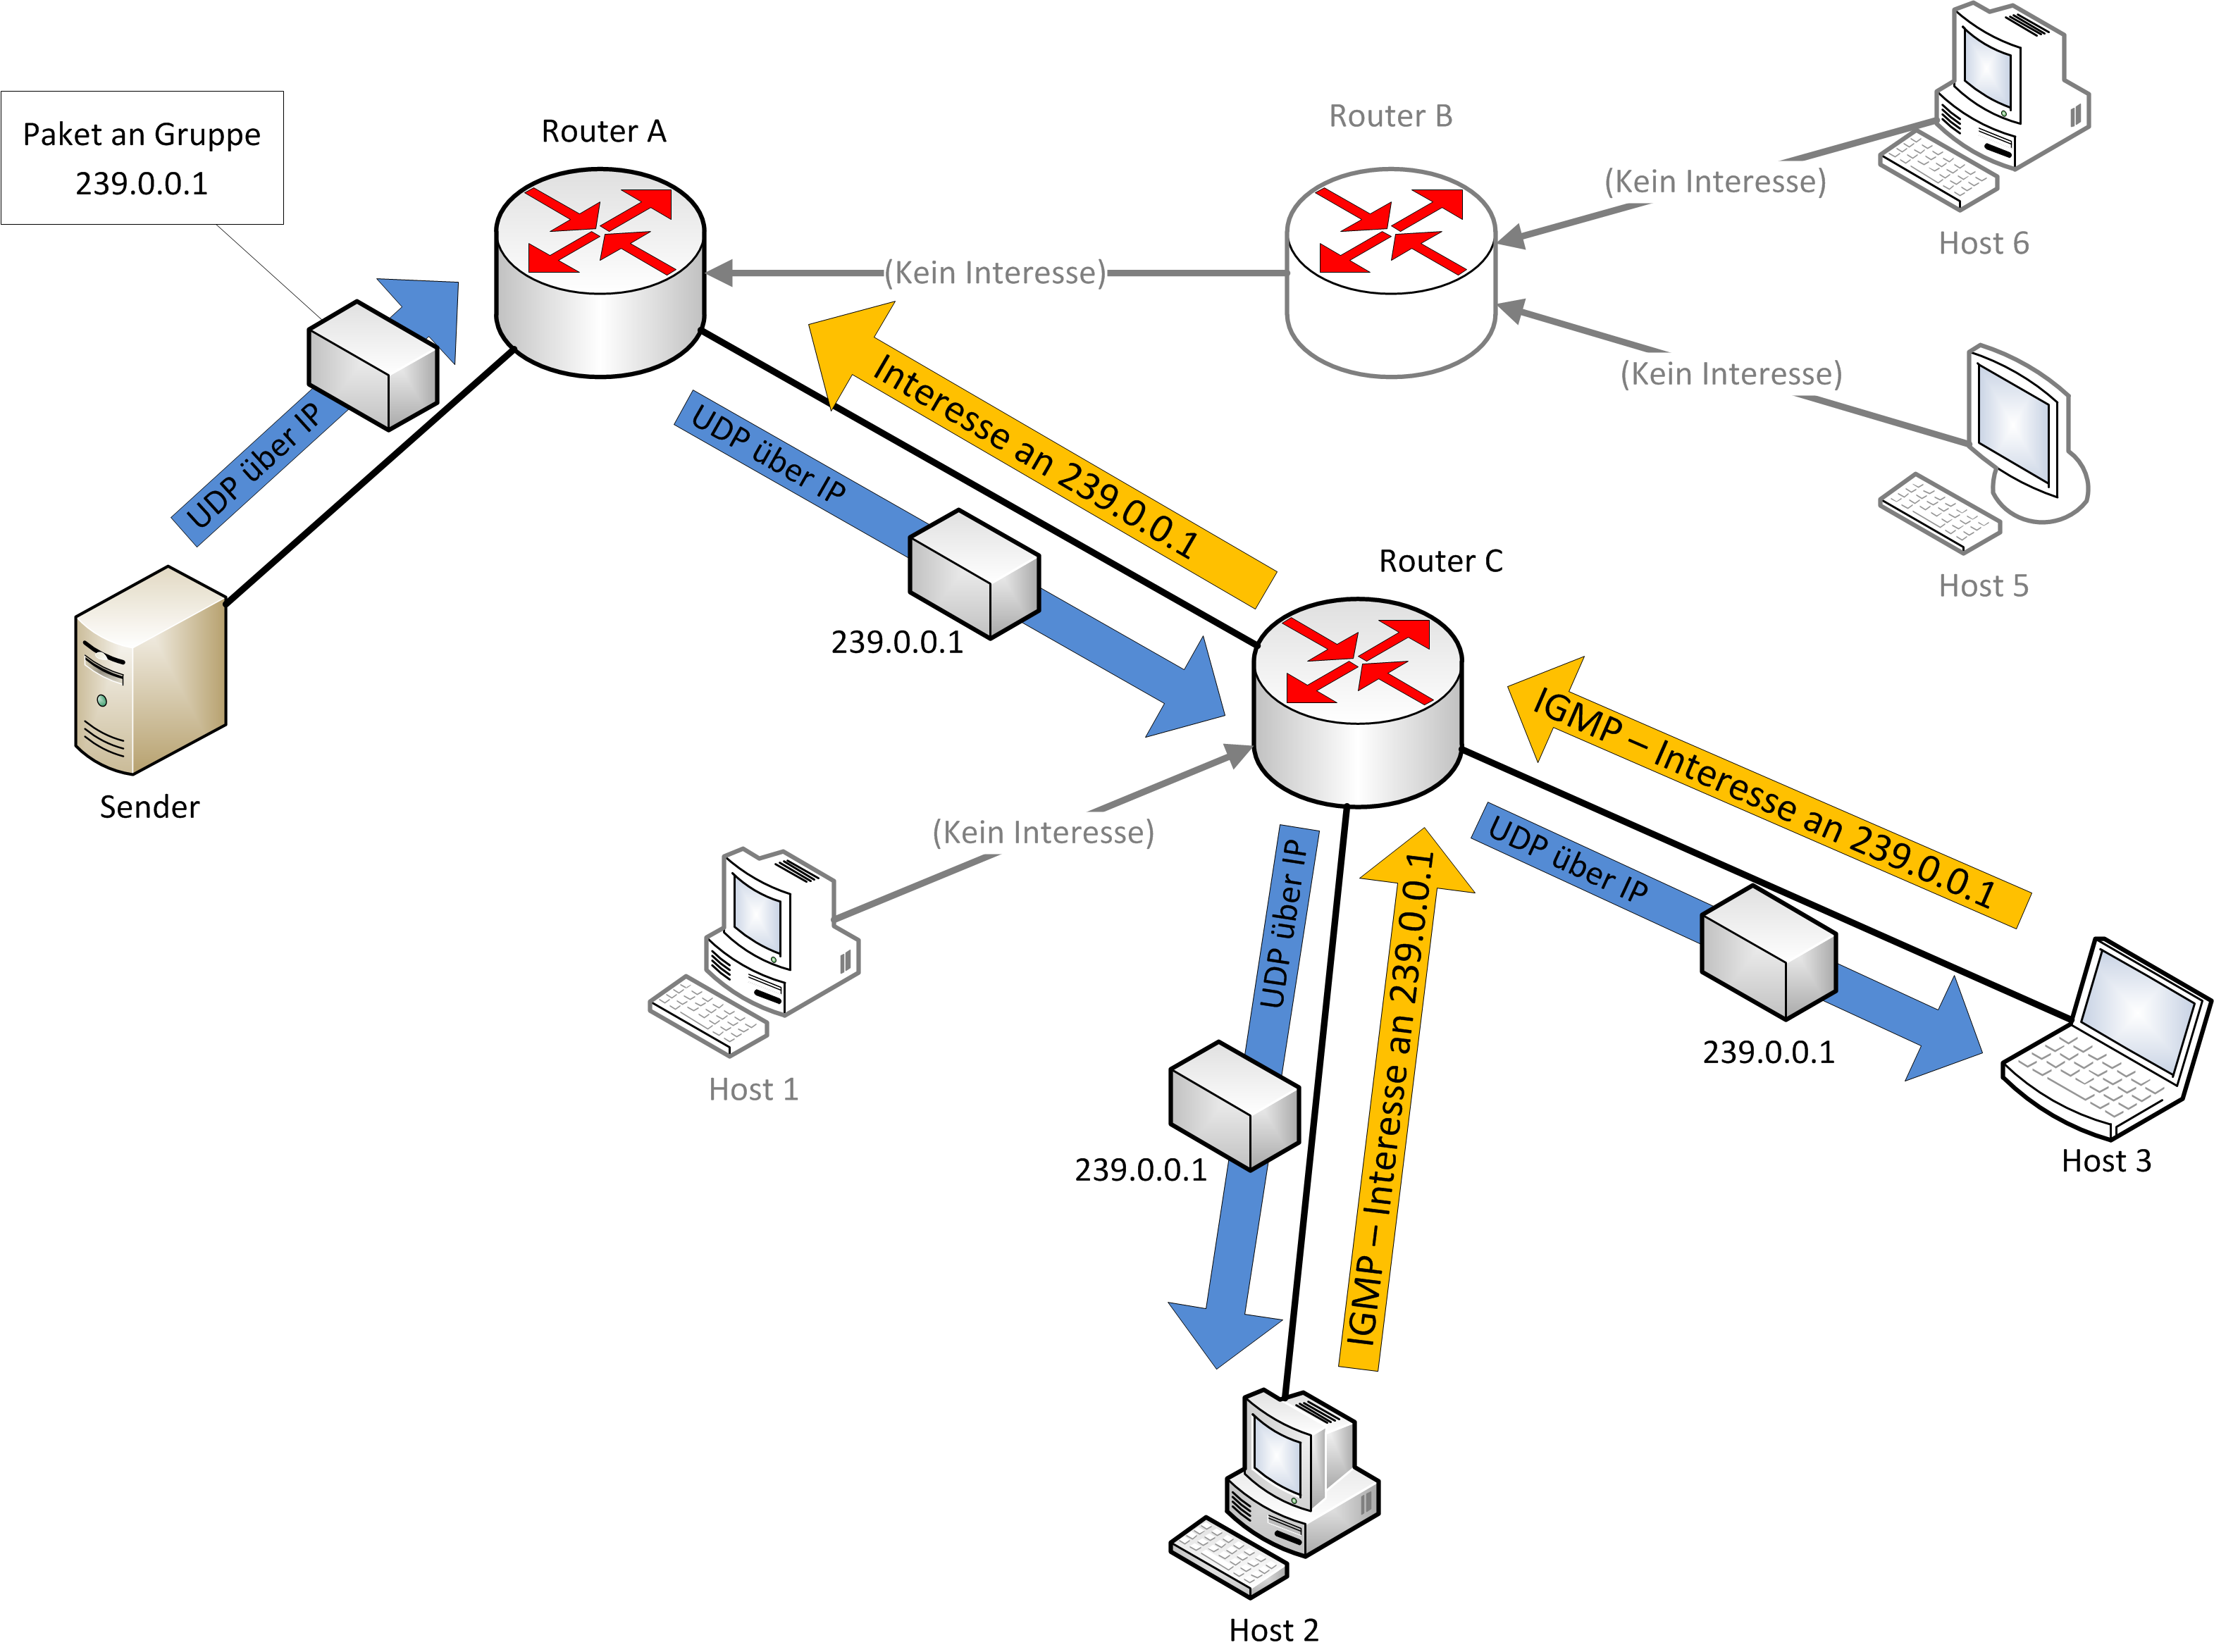
\includegraphics[width=15cm]{images/multicasting.png}
\centering
\caption{Schematische Verteilung eines Multicast-Pakets}
\label{mc_overview}
\end{figure}

Technisch wird Multicasting in OSI-Schicht 3 (Vermittlung/Network) bzw. der ihr
entsprechenden Internetschicht des TCP/IP-Referenzmodells umgesetzt.\\
\\
Wie oben erwähnt, wird Multicast-Datenverkehr durch Multicast-Gruppen und
dazugehörige IP-Adressen organisiert. Auf technischer Ebene heißt das, dass der
Sender in den IP-Header eines Datenpakets nicht die IP-Adresse eines bestimmten
Hosts, sondern eine Multicast-Adresse als Empfänger einträgt. Der
IP-Adressbereich von 224.0.0.0 bis 239.255.255.255 ist für
Multicast-Adressen reserviert (siehe hierfür z.B. RFC3171). Das so erzeugte
IP-Paket wird dann an den nächstgelegenen Router geschickt.\\
\\
Komplexe Multicast-Routing-Protokolle sorgen nun dafür, dass das Paket alle
Router, an die interessierte Hosts angeschlossen sind, erhalten. Um das Netzwerk
nicht unnötig zu belasten, sorgen sie auch dafür, dass Router, deren
angeschlossene Netzwerke überhaupt nicht am Multicast interessiert sind, die
Pakete auch nicht erhalten. Vor Allem muss aber vermieden werden, dass sich in
den Paket-Routen Zyklen bilden, da sie die Leistungsfähigkeit des Netzwerks
stark beeinträchtigen können. Auch wenn die Routing-Protokolle ebenfalls in
OSI-Schicht 3 agieren und \emph{Bestandteil} von IP sind, dienen sie selbst
\emph{nicht} der Datenübertragung. Sie dienen lediglich der Kommunikation der
Router untereinander, damit diese die Multicast-Pakete korrekt weiterleiten
können. Die Multicast-Pakete selber sind nach wie vor gewöhnliche IP-Pakete
(von der speziellen Empfängeradresse im Header abgesehen). Häufig verwendete
Multicast-Routing-Protokolle sind PIM, DVMRP (über IGMP, s.u.) und MOSPF.\\
\\
Um Multicast-Pakete zu empfangen, muss sich ein Host bei einer Multicast-Gruppe
anmelden. Er teilt dazu dem Router, an den er angeschlossen ist mit, dass er an
einer bestimmten Multicast-Gruppe interessiert ist. Die gewünschte
Multicast-Gruppe wird durch ihre Multicast-IP-Adresse spezifiziert. Der Router
weiß nun, dass der angeschlossene Host an allen Paketen interessiert ist, die
diese Multicast-Adresse im Empfängerfeld tragen. Der Host teilt dem Router sein
Interesse über das \emph{Internet Group Management Protocol (IGMP)} mit. Wie
die Routing-Protokolle ist auch dieses Protokoll wieder Teil von IP, dient aber
ebenfalls nicht der Datenübertragung selbst, sondern nur der Kommunikation der Netzwerkknoten
untereinander. Tatsächlich verwendet auch das oben erwähnte DVMRP zum
Informationsaustausch IGMP-Pakete.\\
\\
Das Versenden und Empfangen eines Multicast-Pakets, sowie die dazu
notwendige Interaktion der beteiligten Netzwerkkomponenten ist in Abbildung
\ref{mc_overview} schematisch dargestellt.

\section{Multicasting unter Java}

Die zum Einsatz kommende Java Platform Standard Edition 6 stellt für
Multicast-Anwendungen die \emph{MulticastSocket}-Klasse zur Verfügung. Der
MulticastSocket stellt Methoden zum transparenten Senden und Empfangen von
UDP-Multicast-Paketen bereit. Von der Anwendung werden zum Senden der
Paketinhalt und die Ziel-Gruppenadresse übergeben. Analog wird zum
Empfangen eines Multicast-Streams die gewünschte Gruppenadresse übergeben. Alle
übrigen zur Kommunikation benötigten Systemaufrufe und Mechanismen werden von
der Klasse verborgen. Eine gesonderte Auseinandersetzung mit IGMP oder
Multicast-Routing ist daher auf Anwendungsebene nicht mehr nötig. Aus Sicht des
OSI- und auch des TCP/IP-Schichtenmodells stellt ein Socket damit die Verbindung
zur Transportschicht (OSI-Layer 4) her.

\section{Einordung des Tools}

\begin{figure}[H]
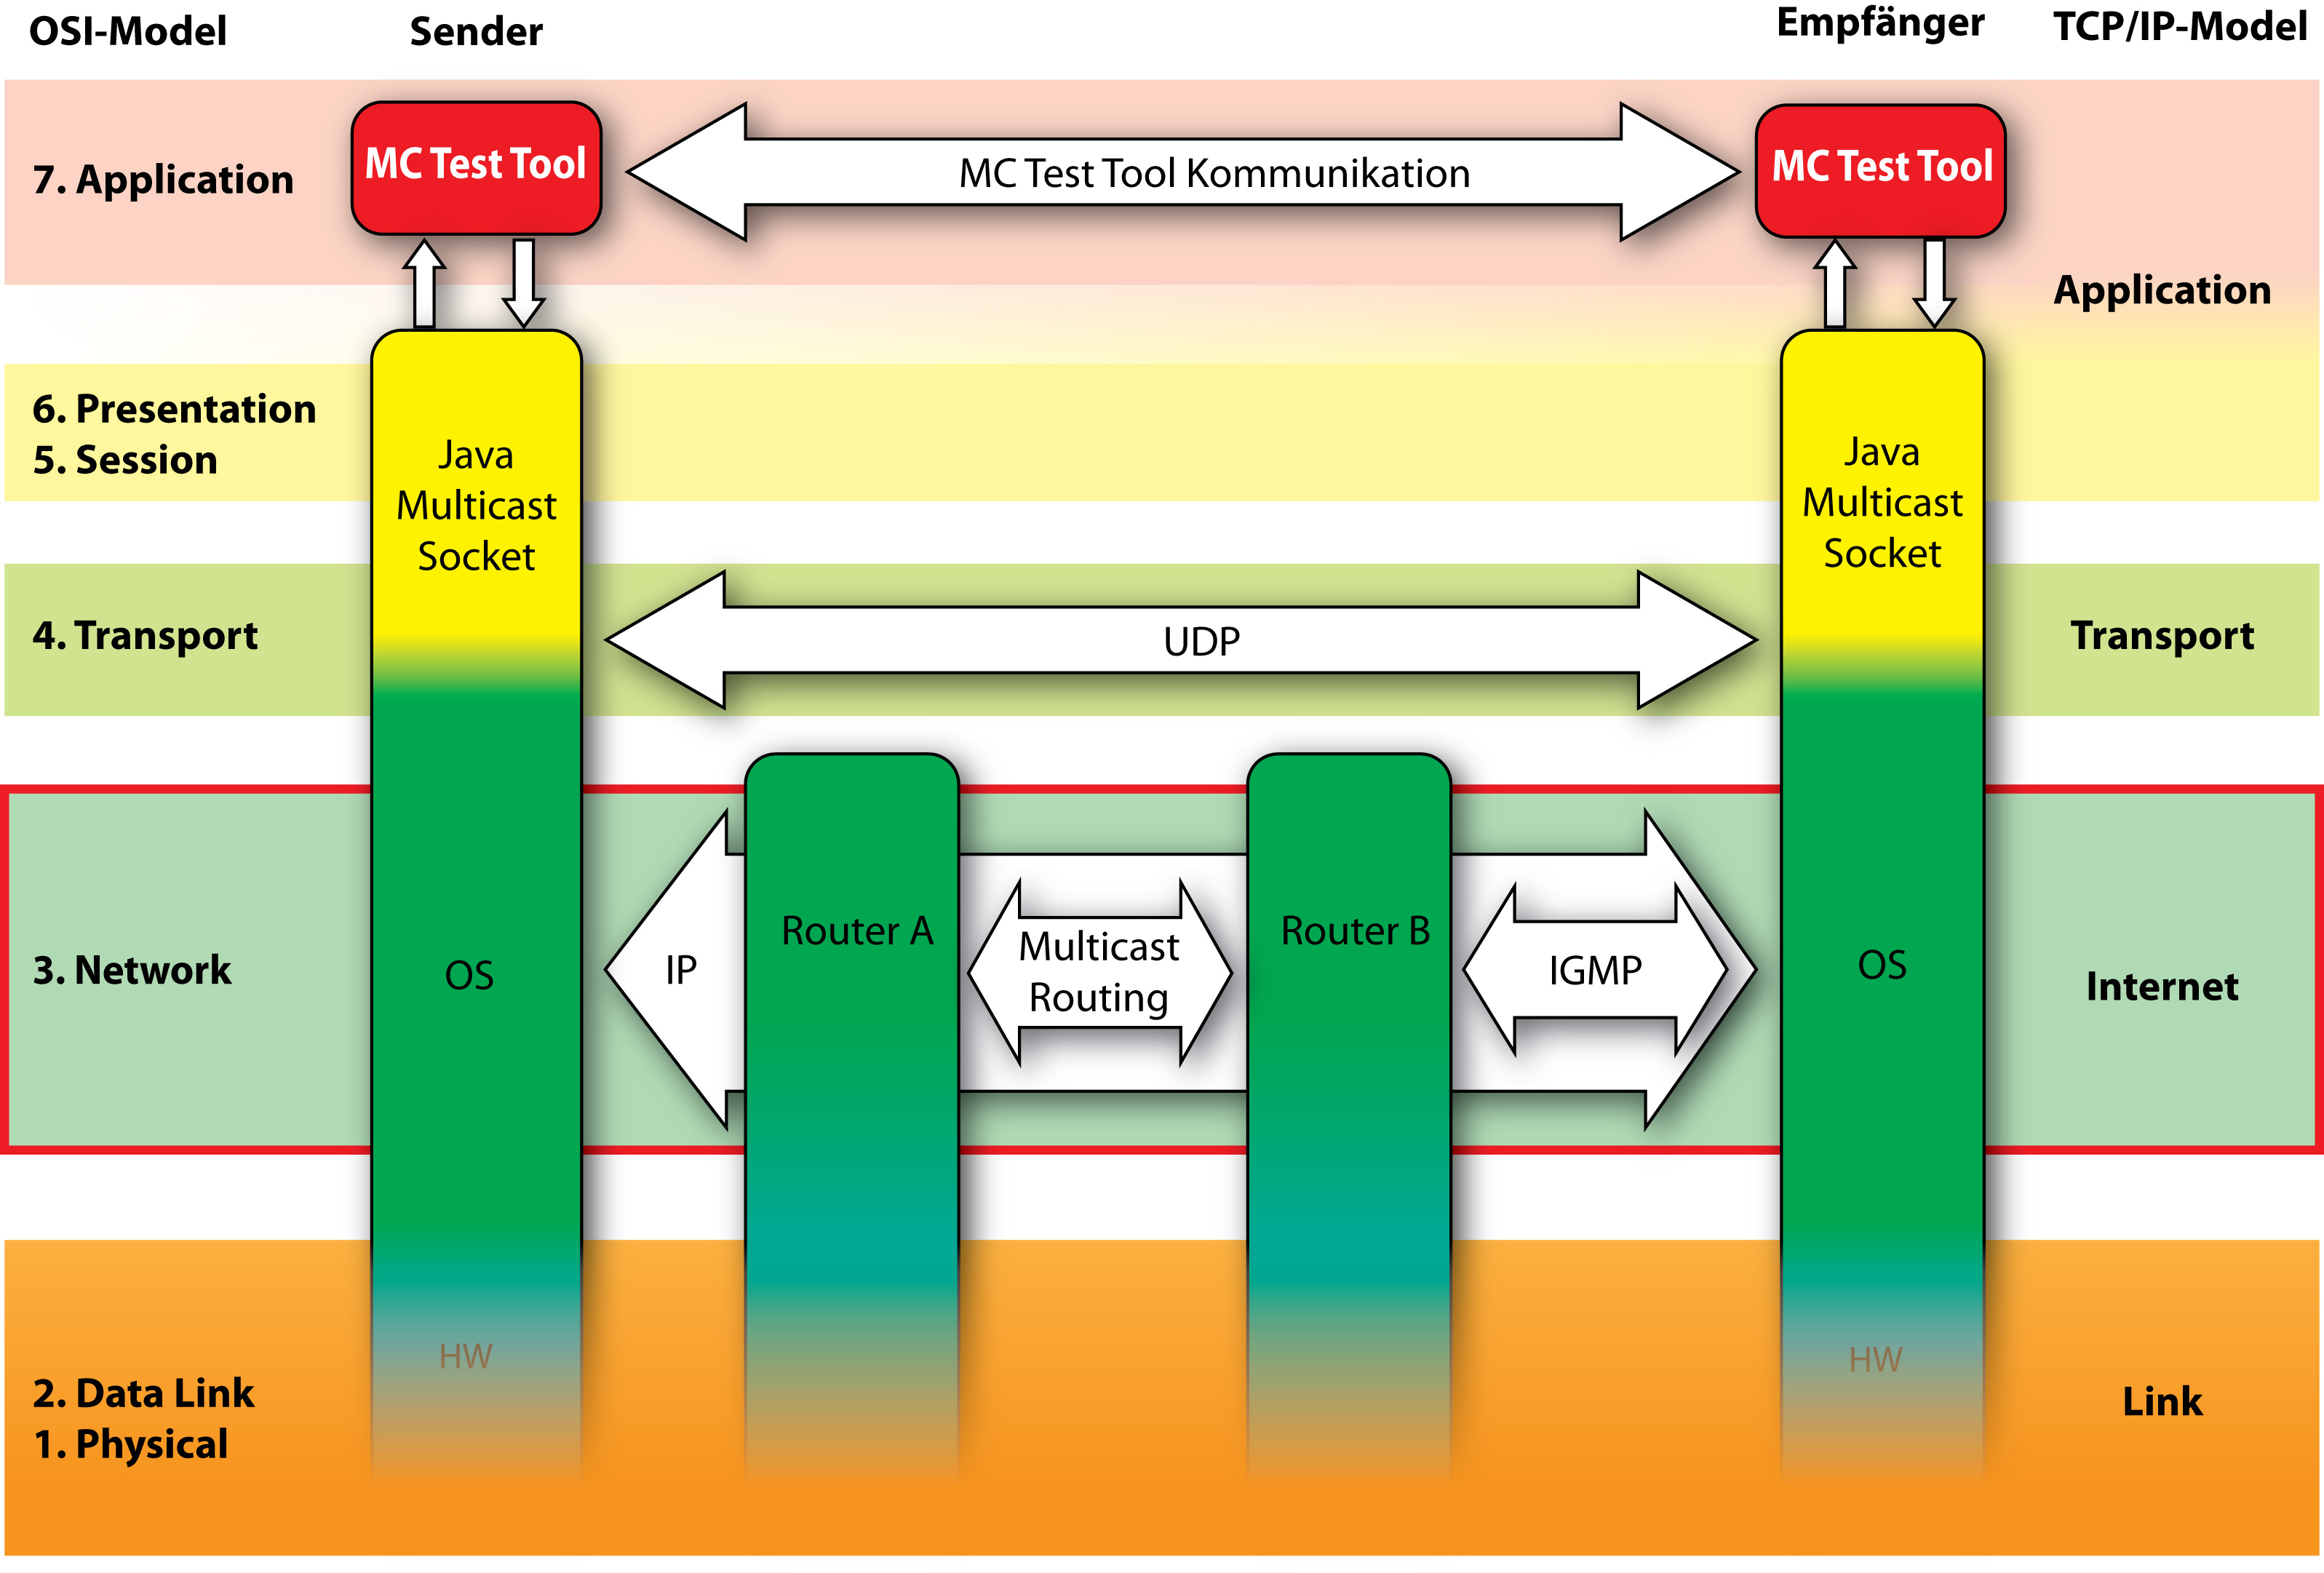
\includegraphics[width=15cm]{images/mc_osi_einordnung.jpg}
\centering
\caption{Einordnung des Gesamtsystems in das OSI- bzw. TCP/IP-Schichtenmodell}
\label{mc_osi_einordnung}
\end{figure}

Hauptaufgabe des Multicast Test Tools ist es, wie bereits beschrieben, die
Multicasting-Fähigkeiten eines Netzwerkes zu testen. Seine Analysen
konzentrieren sich also vor Allem auf die Netzwerkschicht (Schicht 3) des
OSI-Modells bzw. die Internetschicht des TCP/IP-Modells. Den Zugriff auf diese
Schicht stellt der MulticastSocket der Java Platform zur Verfügung. Obwohl also
die Netzwerkschicht Ziel der Untersuchungen ist, wird sich der tatsächliche
Programmieraufwand fast ausschließlich auf die Anwendungsschicht (OSI 7)
konzentrieren.\\
\\
Abbildung \ref{mc_osi_einordnung} gibt einen Überblick über die Einordnung des
Systems ins OSI- bzw. TCP/IP-Modell.

	
	\chapter{Bausteinschicht}
	\label{chap:4}
	Das folgende Kapital beschreibt die statische Grunstruktur des Systems sowie
deren Funktionalität.
{
\bf
Es ist zu beachten, dass sämtliche Diagramme und Beschreibungen in diesem
Abschnitt nur zur Verdeutlichung der Systemarchitektur dienen und noch
keinen Anspruch auf Vollständigkeit erheben. Für alle Arbeiten an einem Modul
ist unbedingt dessen aktuellste Dokumentation zu verwenden.
}

\begin{figure}[H]
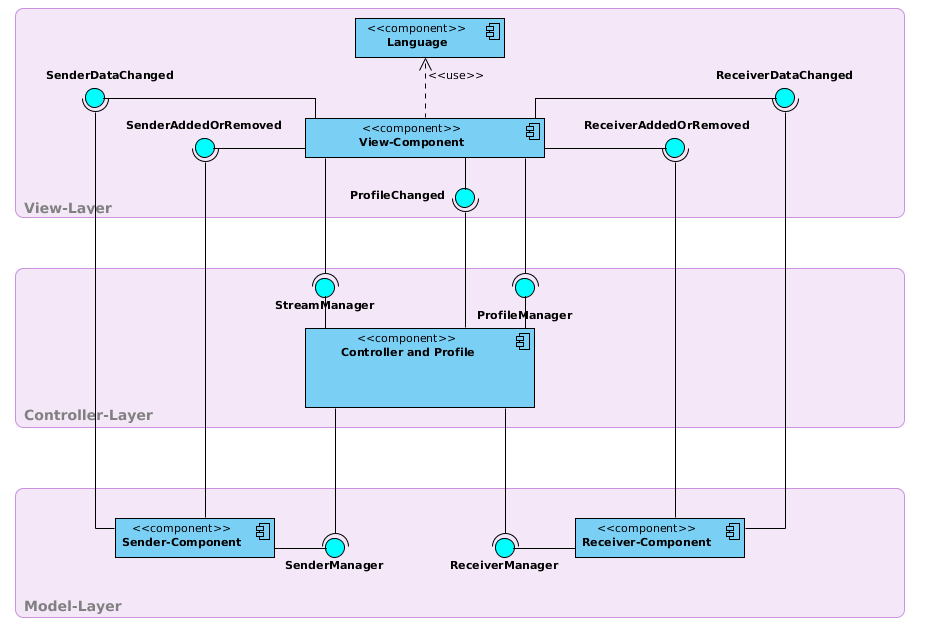
\includegraphics[width=15cm]{images/Overview.png}
\centering
\caption{Komponentendiagramm: Gesamtsystem}
\label{uml_controller}
\end{figure}

Das Gesamtsystem ist zeitgemäß nach dem Model-View-Controller-Entwursmuster
aufgebaut. Dabei werden Programmlogik (Model) und Darstellung (View) voneinander
entkoppelt und kommunizieren über eine Steuerschicht (Controller) miteinander.
Auf diese Weise wird es möglich, die eigentliche Programmlogik direkt für
verschiedene Darstellungsformen zu verwenden. Im Falle des Multicast-Test-Tools
handelt es sich dabei um die graphische Oberfläche (GUI) sowie die
Kommandozeilen-Invokation mit Logger (CLI/Logger). Die graphische Oberfläche ist
weiterhin eingeteilt in einen Darstellungs- und einen Logik-Teil. Die
Anforderung Konfigurationsdateien erstellen und laden zu können, wurde mit den
Profilen des Controllers verwirklicht. Weiterhin wurde das System nach
folgenden Prinzipien modelliert:
\begin{itemize}
  \item Einfache Erweiterbarkeit durch Nutzung des Beobachter-Muster
  (Observer-Pattern) an angemessenen Stellen.
  \item Auslagerung von Logik in eine eigene Klasse nach Strategie-Muster
  (Strategy-Pattern) um Programmfehler durch erwartete, häufige
  Änderungsanfordungen zu vermeiden. Beim MC-Test-Tool wurde das Paketformat auf
  diese Weise in das Paket-Komponente (Packet) ausgelagert.
  \item Geringe Kopplung durch Abstraktion und Schnittstellen-Nutzung.
\end{itemize}

\section{Controller/Profile}
\label{sec:4:steuer}
\begin{figure}[H]
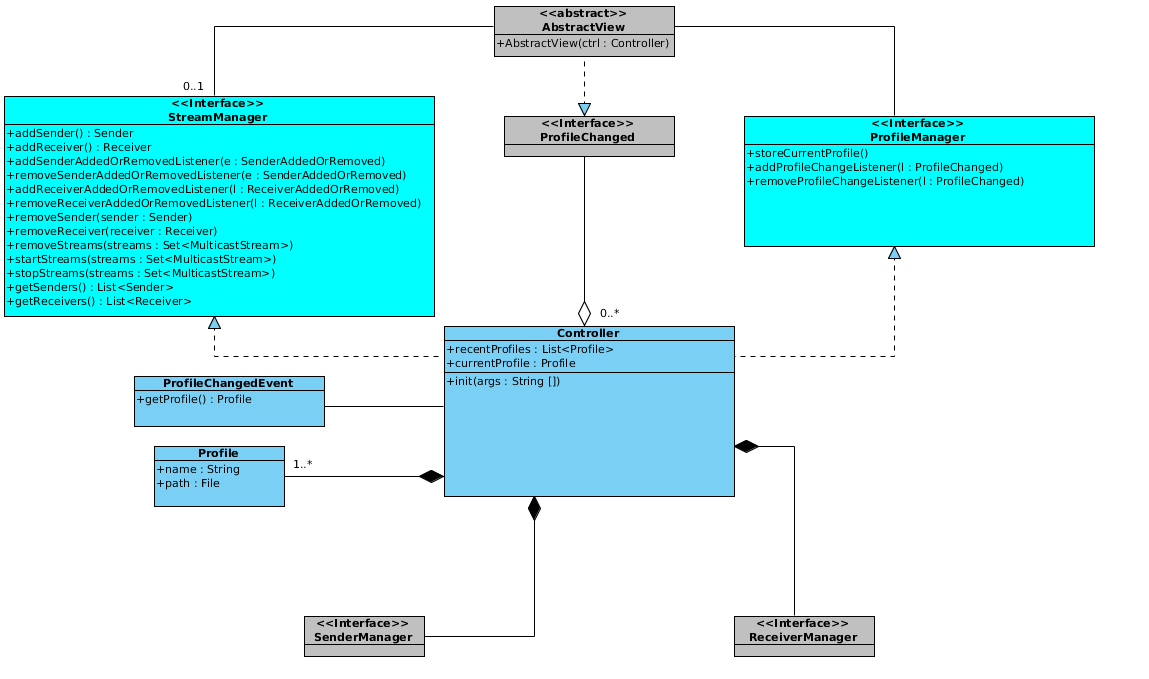
\includegraphics[width=15cm]{images/Controller.png}
\centering
\caption{Klassendiagramm: Controller/Profile - Komponente}
\label{uml_controller}
\end{figure}

\paragraph{Zweck}
Die Controller-Komponente ist der Einstiegspunkt des Systems. Sie erhält beim
Programmstart vom Nutzer alle nötigen Informationen zu dessen Anwendungsabsicht
und entscheidet welche Komponenten auf welche Weise initiliasiert werden müssen.
Danach erstellt sie nach diesen Anforderungen die benötigten Model- und
Viewkomponenten und dient als Kommunikationszentrale zwischen diesen und der
Konfiguration. Die 
\textbf{Profile}-Komponente repräsentiert den Namen und Dateipfad
einer XML-Datei, welche eine mögliche Konfiguration des Programms enthält.
Die Konfigurationsdateien stellen XML-Serialisierungen des momentanen
Controller-Zustands sowie der Ausprägung des Sender- und Receiver-Pools dar.
\paragraph{Erfüllte Anforderungen}
/VA0600/, /QZ10/
\paragraph{Variablität}
volatil - gefestigt
\paragraph{Qualitätsmerkmale}
Änderbarkeit, Anpassbarkeit
\paragraph{Offene Punkte}

\section{Sende- und Empfangsmodul}
\label{sec:4:send}
\begin{figure}[H]
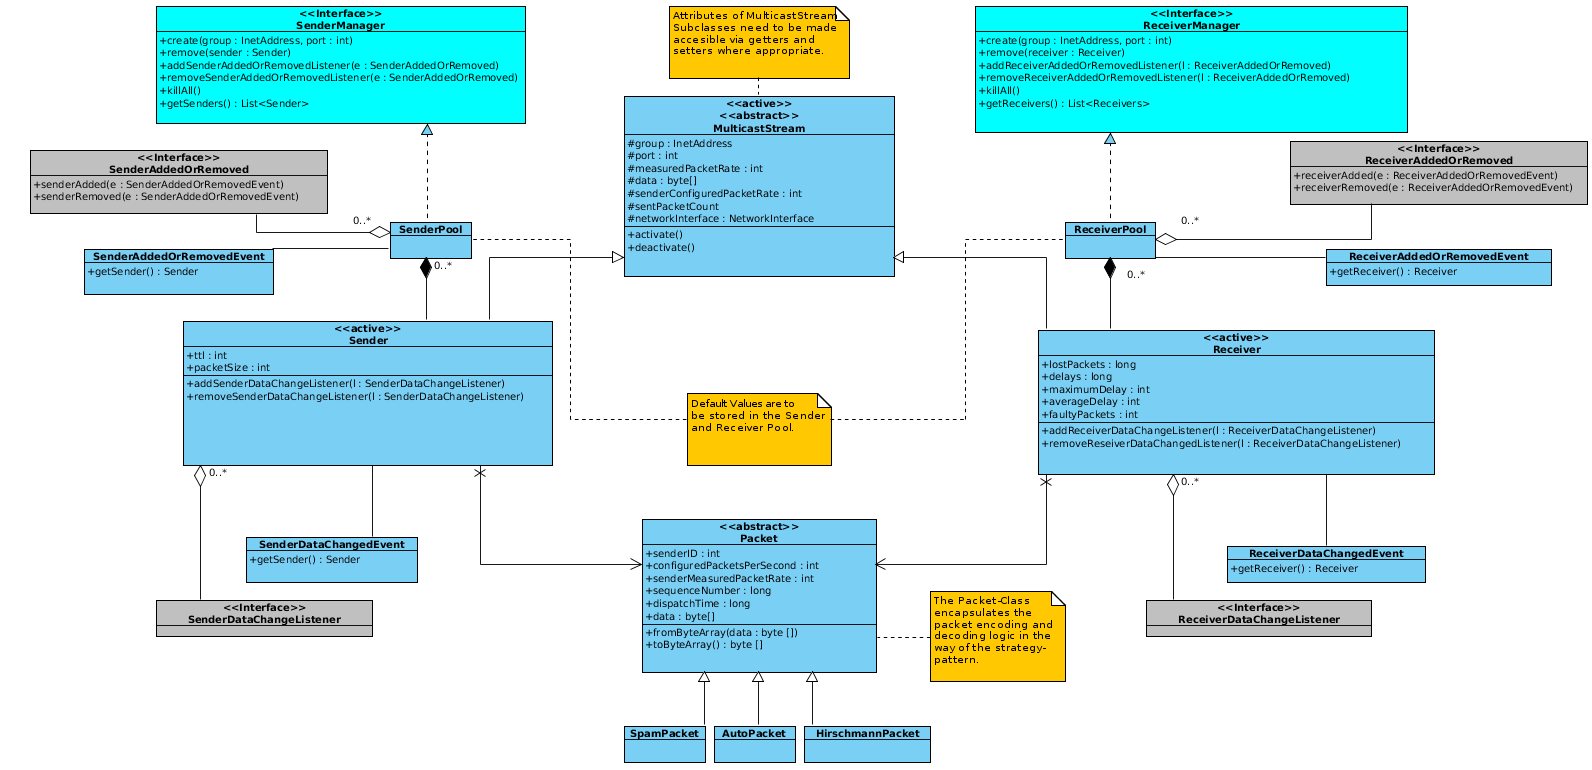
\includegraphics[width=18cm]{images/Model.png}
\centering
\caption{Klassendiagramm: Sende-/Empfangskomponente}
\label{uml_controller}
\end{figure}

\paragraph{Zweck}
Die Sende- und Empfangskomponente des Systems stellt gleichzeitig dessen Kern
dar. Sie besteht aus einer aktiven \textbf{Sender}- und \textbf{Receiver}-Klasse,
die auf Intanzebene jeweils einen sendenden oder empfangenden Datenstrom
repräsentiert. Die Instanzen dieser Klassen arbeiten parallel und autonom in der
Model-Schicht des Systems, erheben alle definierten Daten und informieren alle
Komponenten die die Multicast-Datenstrom Informationen benötigen über die
Schnittstellen \textbf{ReceiverDataChangeListener} und
\textbf{SenderDataChangeListener}. Außerdem existiert jeweils eine
\textbf{SenderPool} und eine \textbf{ReceiverPool} Klasse, die als Container für alle konfigurierten
Datenstrom-Instanzen fungiert und diese verwaltet. Bei Änderungen der
Datenströme, werden interessierte Komponenten über die \textbf{SenderAddedOrRemoved}
bzw \textbf{ReceiverAddedOrRemoved} Schnittstelle benachrichgt.
\paragraph{Erfüllte Andorderungen}
VA0100, VA0200, VA0300, VA0500, VA0800, VA1000, VA1300, OA0100, OA0400
\paragraph{Variablität} gefestigt
\paragraph{Qualitätsmerkmale}
QZ10, QZ30, QZ50, QE10, QP10, QP20, QP40
\paragraph{Offene Punkte}
OP0300 - Verzögerungen?

\section{Paketkomponente}
\label{sec:4:empf}
\begin{figure}[H]
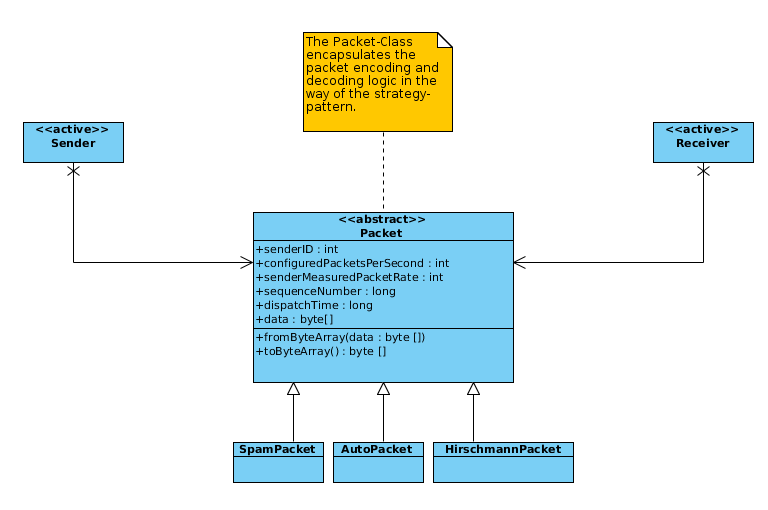
\includegraphics[width=15cm]{images/Package.png}
\centering
\caption{Klassendiagramm: Paketkomponente}
\label{uml_controller}
\end{figure}

\paragraph{Zweck}
Dieses Modul stellt die für die Erkennung und Erstellung von Multicast Paketen 
erforderlichen Funktionalitäten zur Verfügung. Hierbei werden Details über die 
tatsächliche Implementierung des Bitstreams eines Paketes hinter einem 
einheitlichen Interface verbogen. Dies wird unter anderem dadurch erreicht, dass
das Format eines ankommenden Pakets automatisch erkannt wird.
\paragraph{Erfüllte Anforderungen}
/VA0400/, /OA0400/, /QF20/, /QF40/, /QZ20/, /QZ30/, /QZ40/ 
\paragraph{Variablität}
volatil - gefestigt
\paragraph{Qualitätsmerkmale}
Änderbarkeit, Anpassbarkeit, Robustheit
\paragraph{Offene Punkte}

\paragraph{Protokoll Spezifikation}

Um die Testbarkeit eines Multicast Netzwerkes zu ermöglichen, muss das Tool notwendigerweise
Datenpakete via Multicast versenden können. Die versendeten Pakete müssen Informationen über den
Zustand der Applikation zum Zeitpunkt des Versands beinhalten, um so beim Empfänger
Statistiken über die Übertragung erstellen zu können. Um die nötigen Informationen
zu strukturieren ist ein Datenformat von Nöten. Die Struktur sollte einfach
Erweiterbar und trotzdem simpel gehalten sein um das Dekodieren der Pakete 
effizient zu gestalten. Das TLV Protokoll erfüllt all diese Anforderungen.
TLV steht für Type-Length-Value-Format und wird in vielen vorhandenen 
Netzwerkprotokollen, wie zum Beispiel COPS, IS-IS, LLDP und RADIUS genutzt,
wobei es sich dort als erweiterbar und robust bewährt hat.
Bei diesem Protokoll wird jedes Attribut eines Paketes durch folgendes Tripel übermittelt:

\begin{itemize}
 \item[-] Type: bestimmt den Typ des Attributes, in unserem Fall ein unsinged 
                16bit Integer.
 \item[-] Length: bestimmt die Länge des Attribut Wertes und ist 
                  in unserem Fall ein unsigned 32bit Integer.
 \item[-] Value: enthält den eigentlichen Wert des Attributes.
\end{itemize}

Durch die einheitliche Struktur des Protokolls ist es sehr einfach Sequenzen von
TLV Tripel mit einer einheitlichen Funktion zu durchsuchen.
Hierbei werden Tripel mit einem unbekannten Typen ignoriert, was zu einer 
einfachen Erweiterbarkeit führt. Die Anzahl der Tripel im Paket muss nicht 
angegeben werden, da die Länge des Paketes schon im UDP Header enthalten ist.
Zudem kümmert sich UDP auch um die Integrität der Daten, ein extra CRC Hash oder
Paritybits müssen also nicht mit übertragen werden. Alle Datenfelder werden
im Big Endian Format representiert.
\\ \\
Um das hier spezifizierte Protokoll vom Hirschmann-Protokoll und anderen
Protokollen zu unterscheiden, ist ein Header vor den TLV Attributen wichtig. Daher muss vor dem ersten TLV Trippel 
folgendes Hexadezimales Bytemuster stehen.
\\ \\
05 39 00 00 00 00
\\ \\
Diesen Header kann man auch als TLV Trippel mit dem Typ 1337, der Datenlänge
0 und keinen Nutzdaten auffassen. Dieser Umstand vereinfacht potentiell das parsen des Protokolls.
\\ \\
\textbf{Das Protokoll kann wie folgt als DD dargestellt werden:} \\ \\
Paket = Header + {TLV} \\
Header = 0x053900000000 \\
TLV = Type + Length + Value  \\
Type = 0..65535  \\
Length = 0..4294967295 \\
Value = Datenstrom der zuvor genannten Länge. \\
\\ 
\begin{table}[htdp]
\centering
\caption{Im Protokoll verwendete Attribute}
\label{tab:prot}
\begin{tabular}{|l|l|p{9.5cm}|}
\hline
\textbf{Beschreibung} & \textbf{Typ} & \textbf{Attribut Wert} \\
\hline
Sender ID & 1 & Signed 32bit Integer Sender ID.\\
\hline
Eingestellte Paketsenderate & 2 & Pakete pro Sekunde als unsigned 32 bit Integer. \\
\hline
Ermittelte Paketsenderate & 3 & Pakete pro Sekunde als unsigned 32 bit Integer. \\
\hline
Sequenznumber & 4 & Signed 32bit Integer Sequenznumber. \\
\hline
Absendezeit & 5 & Nanosekunden seit dem 1. Januar 1970 00:00 Uhr UTC (vergleiche Unixzeit) als signed 64 bit Integer. \\
\hline
Daten & 6 & Datenstream variabler Länge. \\
\hline
Padding & 7 & Feld zum Auffüllen des Pakets auf eine bestimmte Länge. \\
\hline
\end{tabular}
\end{table}


\section{Language}
\label{sec:4:pakdef}
% uml ausschnitt
\begin{figure}[H]
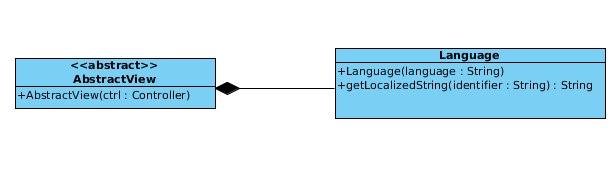
\includegraphics[width=15cm]{images/Language.png}
\centering
\caption{Klassendiagramm: Internationalisierungs-Komponente}
\label{uml_controller}
\end{figure}

\paragraph{Zweck}
In diesem Modul werden alle Internationalisierungsdetails hinter einem sehr einfachen Interface verborgen.
Die Komponente kümmert sich um das laden der Sprachdateien und übersetzt übergebene Template Strings 
in die gewählt Sprache und kümmert sich zudem um die Ersetzung von Platzhaltern in den Strings und
die übersetzung von Exceptions.
\paragraph{Erfüllte Anforderungen}
/QU70/
\paragraph{Variablität}
volatil - gefestigt
\paragraph{Qualitätsmerkmale}
Änderbarkeit, Anpassbarkeit, Simplizität
\paragraph{Offene Punkte}

\section{GUI-Design}
\label{sec:4:konf}
\begin{figure}[H]
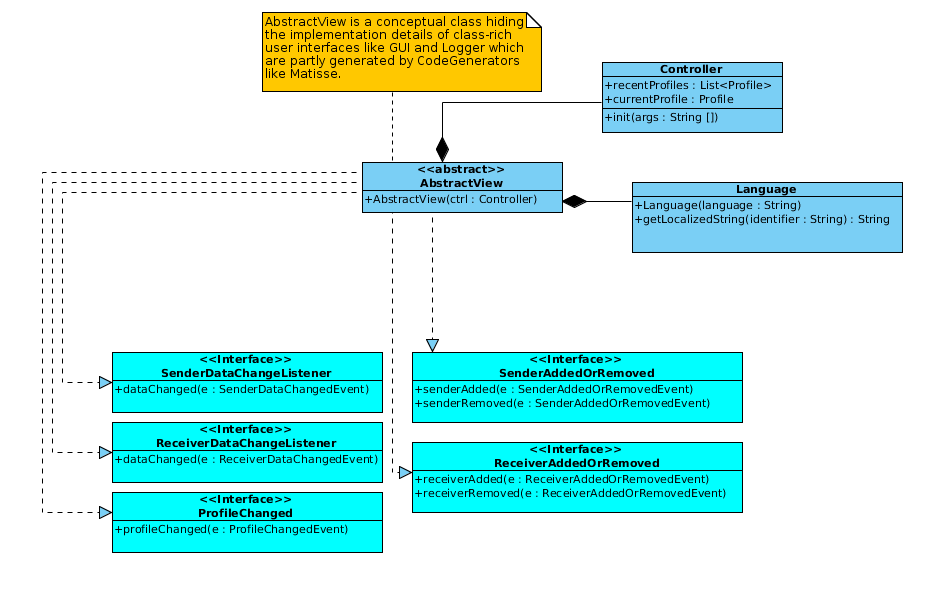
\includegraphics[width=15cm]{images/View.png}
\centering
\caption{Klassendiagramm: View-Komponente}
\label{uml_controller}
\end{figure}

\paragraph{Zweck}
In diesem Modul wird vorallem die konkrete Implementierung der GUI abstrahiert. 
Hierzu gehören beispielsweise die Position von Bedienelementen oder
die Art der Bereitstellung von Benutzeraktionen (Shortcuts, Menüs, Button). 
Dieses Modul hat eine relativ starke Bindung zur Logik der GUI. Ein Model für
eine mögliche Implementierung der GUI ist im Anhang vorhanden. Zu beachten ist
dabei, dass die grafische Darstellung der Datenstromstatistiken nur eine
optionale Anforderung ist.
\paragraph{Erfüllte Anforderungen}
/UC10/, /VA0700/, /VA0800/, /VA1000/, /VA1100/, /VA1200/, /OA0300/, /QF10/, /QU10/, /QU20/, /QU30/, /QU40/, /QU50/, /QU60/
\paragraph{Variablität}
gefestigt
\paragraph{Qualitätsmerkmale}
Änderbarkeit, Anpassbarkeit, guter Look and Feel, Simplizität
\paragraph{Offene Punkte}

\section{GUI-Logik}
\label{sec:4:konf}

\paragraph{Zweck}
Dieses Modul kapselt die Logik der GUI. Hierzu gehört zum Beispiel die 
Umsetzung von Models, welche den einzelnen Swing Komponenten ihre Daten liefern.
Zudem werden hier Konfigurationen gespeichert und geladen.
Dieses Modul hat eine relativ starke Bindung zum Design der GUI. 

\paragraph{Erfüllte Anforderungen}
/UC10/, /VA0700/, /VA0800/, /VA1000/, /VA1100/, /VA1200/, /OA0300/, /QF10/, /QU10/, /QU20/, /QU30/, /QU40/, /QU50/, /QU60/

\paragraph{Variablität}
gefestigt
\paragraph{Qualitätsmerkmale}
Änderbarkeit, Anpassbarkeit
\paragraph{Offene Punkte}

\section{CLI/Logger}
\label{sec:4:konf}

\paragraph{Zweck}
Diese Komponente beinhaltet die Funktionalität, das Programm auf
Kommandozeilenebene zu steuern (im genaueren den Start des Programms mit einer
existieren Konfigurationsdatei und der Definition ob nur die Sendenden,
Empfangenden oder alle Datenströme geladen werden sollen). Dies umfasst die
Definition und Dokumentation des Kommandozeilenaufrufs sowie die Implemtierung
der \textbf{ArgumentParser}-Klasse, die eine Reihe von Kommandozeilenargumenten
in dieser Hinsicht interpretiert. Die Logger-Funktionaltität muss als
View-Komponente implementiert werden. Sie erhält damit von den Datenströmen
regelmäßig statistische Informationen und muss diese in einer Log-Datei
persistieren.
\paragraph{Erfüllte Anforderungen}
/UC20/, /VA0900/, /QF30/
\paragraph{Variablität}
volatil
\paragraph{Qualitätsmerkmale}
Änderbarkeit
\paragraph{Offene Punkte}
Log-Format als Fließtext, XML oder konfigurierbar?\\
Detailierung\\

\section{Installer}
\label{sec:4:konf}
\paragraph{Zweck}
Einfache Installation unter Windows und Linux Debian.
\paragraph{Erfüllte Anforderungen}
/QP30/
\paragraph{Variablität}
volatil
\paragraph{Qualitätsmerkmale}
Einfache Bedienbarkeit
\paragraph{Offene Punkte}
Je nachdem Java WebStart?

	
	\chapter{Laufzeitschicht}
	\label{chap:5}
	%TODO @Konne,Jeff

\section{Starten der Applikation}
\label{sec:5:startapp}
\begin{figure}[H]
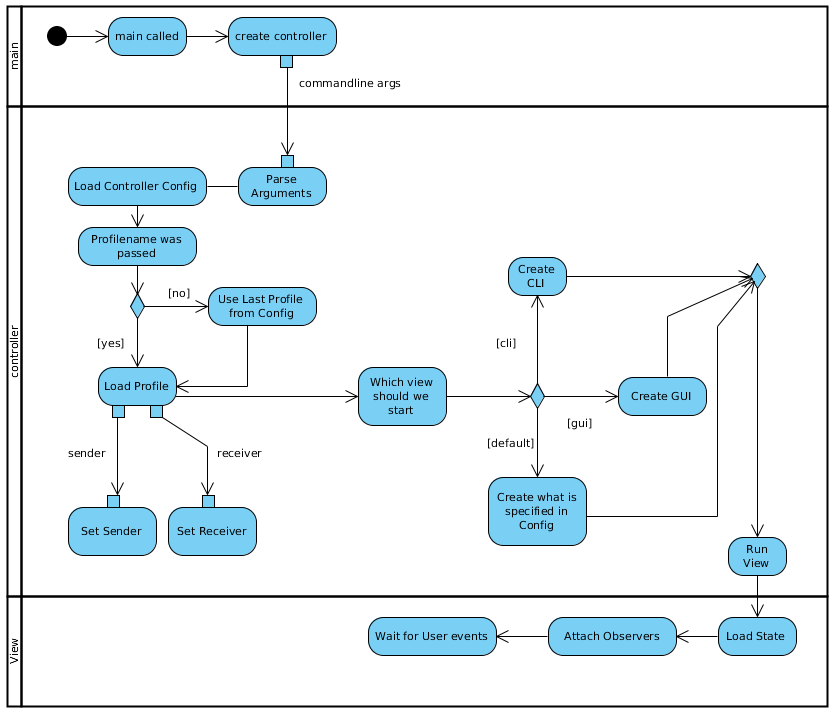
\includegraphics[width=15cm]{images/Init.png}
\centering
\caption{Starten der Applikation - UML Activity Diagramm}
\label{fig_init}
\end{figure}

Zeigt die Initialisierung der Applikation. Hierzu gehört das Parsen der
übergebenen Argumente, das Laden eines Profils und die Erstellung und 
Ausführung einer View.

\section{Beenden der Applikation}
\label{sec:5:stopapp}
\begin{figure}[H]
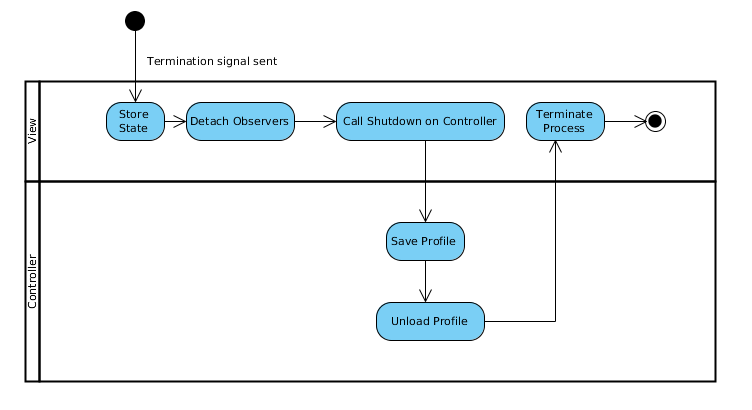
\includegraphics[width=15cm]{images/Shutdown.png}
\centering
\caption{Beenden der Applikation - UML Activity Diagramm}
\label{fig_shutdown}
\end{figure}

Zeigt wie die Applikation zu beenden ist, so dass sie sich auch danach
noch in einem konsistenten Zustand befindet.

\section{Profil Laden}
\label{sec:5:loadprofile}
\begin{figure}[H]
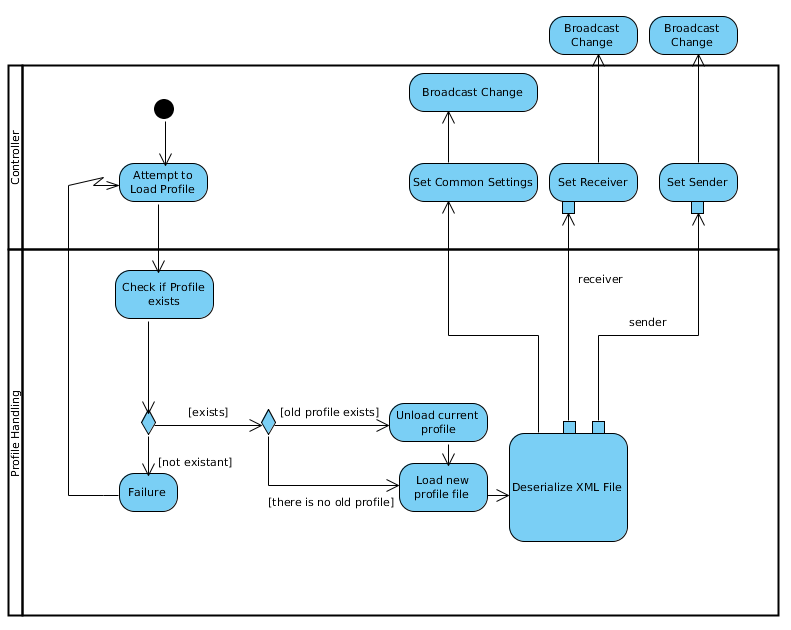
\includegraphics[width=15cm]{images/LoadProfile.png}
\centering
\caption{Profil Laden - UML Activity Diagramm}
\label{fig_loadprofile}
\end{figure}

Zeigt wie ein Profil geladen wird. Dies geschieht zum Beispiel beim
Start der Applikation und nach dem schließen eines anderen Profils.
Nach der Deserialisierung wird das System über die Änderungen im Profil
informiert.

\section{Profil Speichern}
\label{sec:5:loadprofile}
\begin{figure}[H]
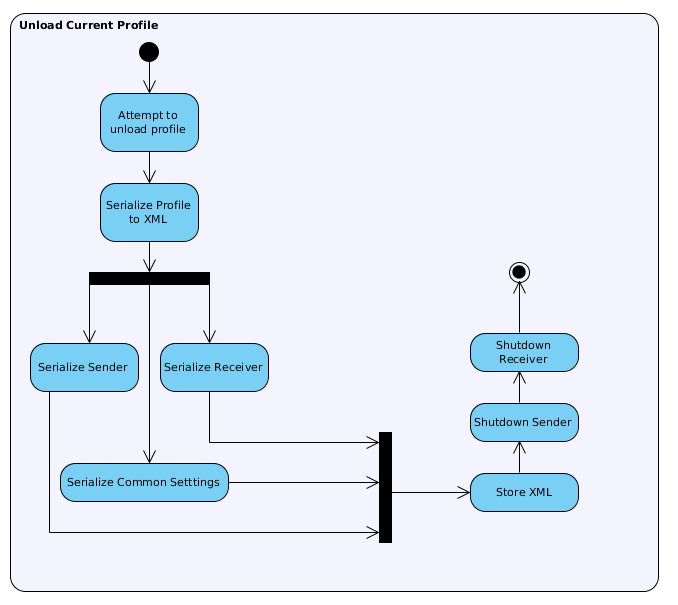
\includegraphics[width=15cm]{images/UnloadProfile.png}
\centering
\caption{Profil Speichern - UML Activity Diagramm}
\label{fig_unloadprofile}
\end{figure}

Bei der Speicherung und dem Schließen eines Profils werden alle 
wichtigen Komponenten serialisiert und danach heruntergefahren.

\section{Empfang eines Multicast-Pakets}
\label{sec:5:recmc}
\begin{figure}[H]
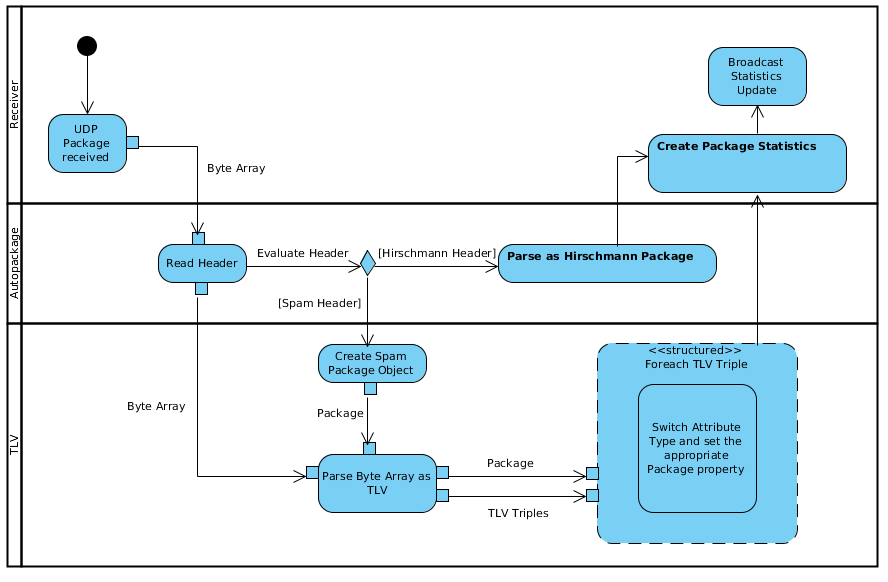
\includegraphics[width=15cm]{images/Receive.png}
\centering
\caption{Empfang eines Mutlicast-Pakets - UML Activity Diagramm}
\label{fig_receive}
\end{figure}

Hier wird beschrieben wie ein Spam Multicast Paket empfangen und
dann in ein Objekt umgewandelt wird.

\section{Automat der Empfangseinheit}
\label{sec:5:recmc}
\begin{figure}[H]
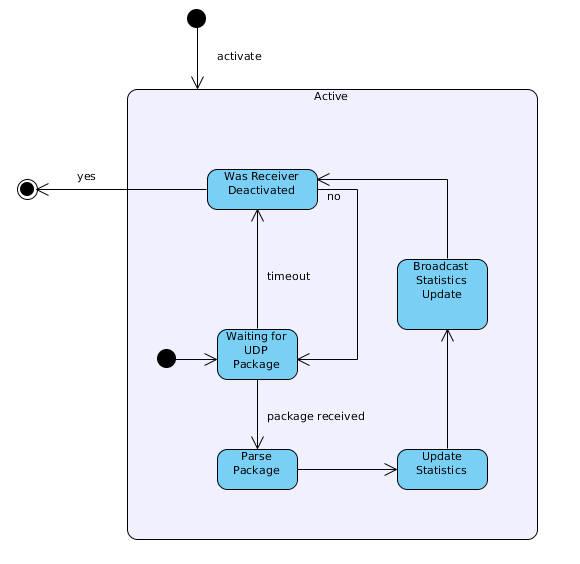
\includegraphics[width=15cm]{images/ReceiveState.png}
\centering
\caption{Automat der Empfangseinheit - UML Automat}
\label{fig_rcvstate}
\end{figure}

Dieser Automat beschreibt wie die Empfangskomponente auf das Empfangen
von Paketen wartet.

\section{Interaktion zwischen View, Sender und Empfänger}
\label{sec:5:readconf}
\begin{figure}[H]
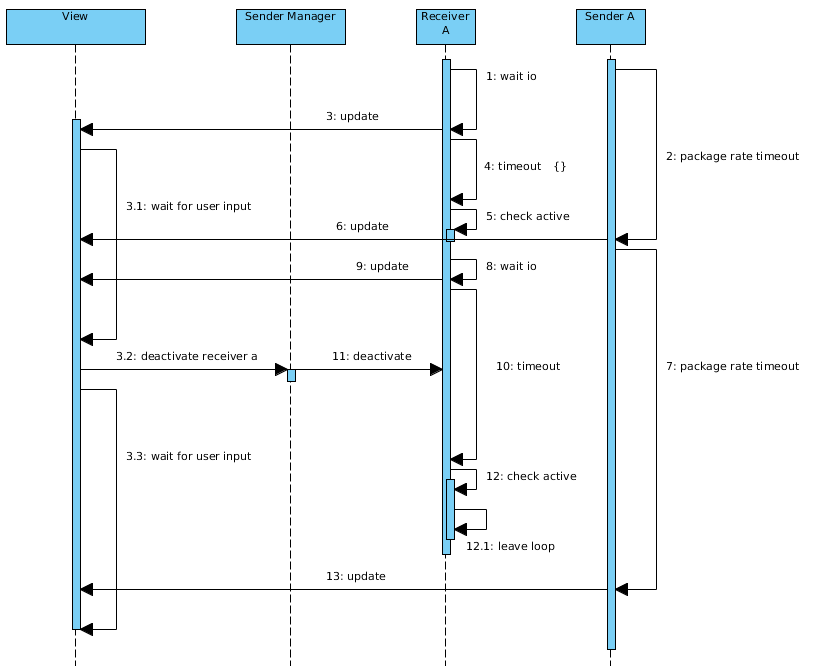
\includegraphics[width=15cm]{images/Threads.png}
\centering
\caption{Interaktion zwischen View, Sender und Empfänger - UML Sequence Diagramm}
\label{fig_threads}
\end{figure}

Dieses Sequenzdiagramm zeigt die Interaktion zwischen einer View und
dem Sender und Receiver. Hiermit wird die Observerstruktur und die
Nebenläufigkeit der einzelnen Komponenten veranschaulicht.

	
	\chapter{Technische Konzepte}
	\label{chap:6}
	%TODO Faseln
\section{Persistenz}
\label{sec:6:pers}
\subsection{Konfiguration}
Gemäß VA0050 und VA0060 (siehe SRS) muss das System alle konfigurierbaren
Parameter in einer XML-Datei sichern. Für diese XML-Datei wird ein eigener DTD
erstellt. Die Semanthik muss ausdrucksstark genug sein, um eine einfache,
manuelle Bearbeitung zu ermöglichen.

\subsection{Logging}
Hinsichtlich VA0900 und VA1300 (siehe SRS) bietet das System die Möglichkeit
eine Logger-Komponente zu aktivieren, die alle definierten Statistiken über die
Datenströme in einer XML-Datei speichert.

\section{Nutzeroberfläche}
\label{sec:6:ober}
\subsection{Graphisch}
Nach VA0700 und VA0800 muss das gesamte System über eine graphische
Nutzeroberfläche gesteuert werden können. Diese wird in Swing entweder manuell
oder mit GUI-Buildern wie Mantisse erstellt. Ein Prototyp mit den minimalen
Anforderungen ist in Anhang \ref{a:gui} ersichtlich.

\subsection{Textuell}
Das System muss nach VA0900 die Möglichkeit bieten, über die Kommandozeile eine
Konfigurationsdatei zu laden und im Hintergrund zu arbeiten.

\section{Ergonomie}
\label{sec:6:ergo}
\subsection{Performanz}
Keine Nutzerinteraktion darf mehr als 100ms benötigen, bis dass der Nutzer eine
Rückmeldung vom System bekommt.\\
Beim gleichzeitigen Betrieb von 30 Datenströmen dürfen
bei einem handelsüblichen Rechner mit 2,4GHz Intel Core 2 Duo Prozessor und 2GB RAM nicht mehr als 80\%
des Systems ausgelastet werden.

\subsection{Benutzerfreundlichkeit}
Die graphische Nutzeroberfläche muss es ermöglichen, mehre Datenströme
gleichzeitig zu aktivieren, zu deaktiveren und in sinnvollen (nicht
Datenstrom-spezifischen wie Port, Gruppe, \ldots) Attributen zu ändern.\\
Die definierten Daten, die über jeden Datenstrom erhoben werden, müssen auf
einen Blick ersichtlich sein.

\subsection{Automatisierbarkeit}
Das System muss per Kommandozeilenschnittstelle in Skripten eingebunden werden
und im Hintergrund arbeiten können.

\section{Verteilung, Kommunikation mit anderen Systemen, Migration}
\label{sec:6:komm}
Mehrere, voneinander funktional-unabhängige Instanzen des Systems können auf
vielen verschiedenen Knoten eines Netzwerks in Betrieb genommen werden können. Diese
kommunizieren dabei untereinander oder mit dem alten
System der Hirschmann Automation GmbH.

\section{Parallelisierung}
\label{sec:6:para}
Die einzelnen Datenströme werden mit den Mitteln der Java-Plattform
parallelisiert. Die Java-Virtual-Machine entscheidet weiterführend, wie die
Parallelisierung auf Rechner-Ebene umgesetzt wird.

\section{Internationalisierung}
\label{sec:6:inter}
Die Nutzeroberflächen und Ausgaben müssen international betextbar sein. Mit der
Endversion der Software werden die Sprachen Deutsch und Englisch ausgeliefert.
Weiter Sprachen müssen einfach mit Klartext-Dateien hinzugefügt werden können.

\section{Codeverwaltung, Build-Management und Testing}
\label{sec:6:bm}
Der Quelltext des Projektes wird auf dem Unternehmensserver in einem zentralen
Mercurial-Repository verwaltet. Gebaut wird nach Continuous-Integration Prinzip
mit Apache Maven und Apache Continuum als Weboberfläche. Komponententests
werden automatisch mit jedem Build per JUnit V4.8.* durchgeführt, ebenfalls
durch Maven.

	
	\chapter{Entwurfsentscheidungen}
	\label{chap:7}
	%El Konno
%Design Patterson begründen
%MVC,Factory, Strategy, Observer

\section{Gesamtsystem}
\label{sec:7:global}

Das Gesamtsystem wird zur besseren Verständlichkeit und zur Vermeidung von Abhängigkeiten 
in logische Komponenten unterteilt. \\
Auf höchster Abstraktionsebene ist das strukturgebende Element der Anwendung ein Model-View-Controller Pattern.
Dieses Pattern gliedert die Applikation in drei Untermodule, das Model, die View und den Controller.
Die Entscheidung dieses Pattern zu benutzen fiel auf Grund der vielen architektonischen Vorteile.
So herrscht zwischen den einzelnen Komponenten eine strenge Hierarchie. Das Model weiß von keinem Controller und
der Controller kennt keine View. Durch diese Trennung besteht eine sehr schwache Kopplung zwischen den einzelnen
Komponenten. Zudem lässt sich die View sehr flexibel gestalten und es können sogar mehrere Views zur gleichen
Zeit aktiv sein, ohne sich gegenseitig zu stören. Diese Flexibilität der View ist ausschlaggebend für 
die Anpassungsfähigkeit der Applikation an ein sich änderndes Umfeld. Die tatsächliche Lösung des Problems 
behält nämlich meistens über einen relativ langen Zeitraum seine Berechtigung, während sich die Anforderungen
an die Visualisierung und Bedienung der eigentlichen Programmlogik viel schneller ändern. 
Aber der wohl wichtigste Grund ist die Bewährtheit des Patterns. So wird er von den meisten modernen Applikationen
umgesetzt und findet sich auch in jeder modernen GUI Library wieder. Der einzige Nachteil des Patterns sind
Performance Einbusen, wie sie bei den meisten Ansätzen der architektonischen Strukturierung anfallen.

\section{Paket Protokolle}
\label{sec:7:packet}
Um die relevanten Daten aus den UDP Paketen zu extrahieren wird ein Strategy Pattern verwendet.
Dieses Pattern verbirgt den Algorithmus zum parsen des Pakets aus dem UDP Bitstream hinter einem von der
Implementierung unabhängigen Interface.

\section{Serialisierung}
\label{sec:7:serial}
An die aspektorientierte Programmierung angelehnt, ist die gesamte
Serialisierung von Daten, welche persistent gemacht werden müssen, in einen Teil des Controllers ausgelagert.

\section{Benutzer Interaktion}
\label{sec:7:user}
Das Model und der Controller bilden zusammen eine vollständige Lösung um ein
Netzwerk auf Multicastfähigkeit zu testen. Die View soll nur die Interaktion eines Benutzers mit der Lösung vereinfachen. Dieser Ansatz führt zu einem
hohen Wiederverwendungsgrad der Lösung des tatsächlichen Problems. Man könnte einfach mit den Komponenten des
Controllers und des Models linken und so die komplette Lösung in eine eigene Applikation integrieren. 
Da Sprache nur bei der Bedienung von Menschen von Relevanz ist, ist die Komponente zur Internationalisierung 
auch nur in der View implementiert.


	
	%\chapter{Architekturbewertungs-Kriterien}
	%\label{chap:8}
	%\section{Leistungsfähigkeit}
%TODO abstrakt mit genauen Zahlen
%  Begründung warum die Architektur gut ist
\label{sec:8:leistung}
\paragraph{Auslöser} Nutzer startet 30 sendende und empfangende Mutlicastströme
gleichzeitig
\paragraph{Quelle} interner Nutzer
\paragraph{Systemzustand} Normallast
\paragraph{Antwort} normale Funktion
\paragraph{Metrik} Nicht mehr als 80\% CPU-Auslastung mit handelsüblichem 2,4GHz
Dual-Core Prozessor.

	
	\chapter{Projektaspekte}
	\label{chap:9}
	%TODO @Dave Überblick
\section{Änderungsaufträge}
\label{sec:9:change}

Während der Implementierungsphase werden in diesem Abschnitt die Änderungsaufträge dokumentiert. 
Die Liste ist von den beiden Systemarchitekten nach Rücksprache mit dem Projektmanager zu aktualisieren.

\begin{table}[htdp]
\caption{Änderungsaufträge}
\label{tab:aenderung}
\begin{center}
\begin{tabular}{|p{2cm}|p{3cm}|p{4.5cm}|p{5cm}|}
\hline
\textbf{Id} & \textbf{Komponente} & \textbf{Änderung} & \textbf{Beschreibung} \\
\hline
&&&\\
\hline
\end{tabular}
\end{center}
\label{default}
\end{table}

\section{Technische Risiken}
\label{sec:9:techrisk}

\section{Offene Punkte}
\label{sec:9:offen}

Die folgende Tabelle enthält offene Punkte, die wärend der Implementeirungsphase, wenn möglich noch davor, geklärt werden müssen.

\begin{table}[htdp]
\caption{Offene Punkte}
\label{tab:offeneP}
\begin{center}
\begin{tabular}{|p{2cm}|p{5cm}|p{8cm}|}
\hline
\textbf{Id} & \textbf{Kurzbeschreibung} & \textbf{Beschreibung}\\
\hline
 /OP0100/ & Optionale Anforderungen & Welche optionalen Anforderungen können noch realisiert werden?\\
\hline
 /OP0200/ & User Interface & Sollen "`Docklets"' zur Gestaltung verwendet
 werden?\\
 \hline
 /OP0300/ & Daten & Was ist mit Verzögerungen gemeint?\\
\hline
\end{tabular}
\end{center}
\label{default}
\end{table}

\section{Erwartete Änderungen}
\label{sec:9:erw}

Es wurden keine zu erwarteten Änderungen registriert, da der Kunde intensiv in die Requirements Engineering-Phase eingebunden wurde.

\section{Migration}
\label{sec:9:mig}

Das bisherig verwendete Programm der Hirschmann Automation GmbH soll durch das zu entwickelnde Produkt ersetzt werden.\\
Um einen fließenden Übergang bei der Migration zu schaffen, soll das Programm in der Lage sein die Datenströme des bisher verwendeten Programms
zu empfangen und auszuwerten. Hingegen muss die Empfangsfähigkeit auf der Seite des Hirschmann Tools nicht gewährleistet werden.\\
Bei der Architektur ist somit unbedingt darauf zu achten, dass das entsprechende Protokoll erkannt und unterstützt wird.
	
	\begin{appendix}

	\chapter{Grafische Nutzeroberfläche}
\label{a:gui}

%\section{Verwendete Abk"urzungen}

\begin{figure}[H]
\centering
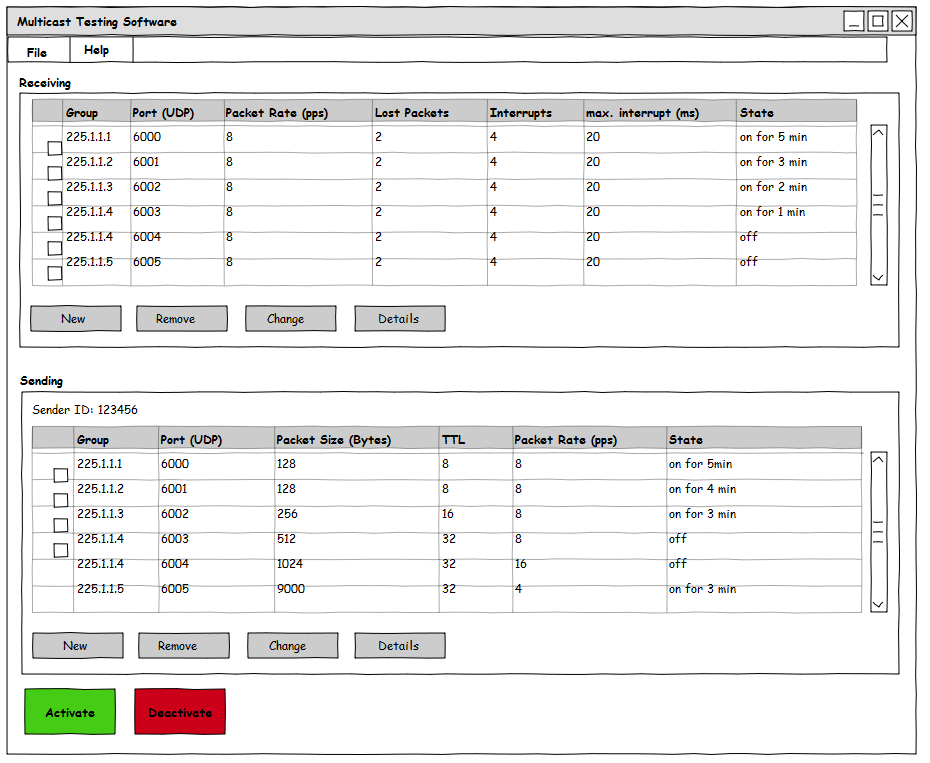
\includegraphics[scale=0.5]{images/gui/main.png}
\caption{Hauptprogramm}
\end{figure}
Die Standart-Ansicht des Programms zeigt eine Auflistung aller aus- und
eingehenden Datenströme. Nach Anforderungen werden alle relevanten
Informationen auf einen Blick angezeigt und es können bequem mehrere Ströme auf
einmal bearbeitet werden.

\begin{figure}[H]
\centering
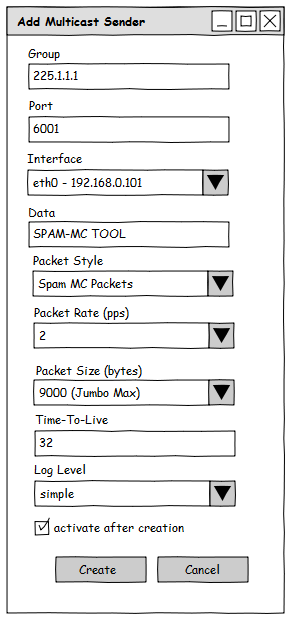
\includegraphics[scale=0.5]{images/gui/addsender.png}
\caption{Hinzufügen eines Senders}
\end{figure}
Beim Hinzufügen eines neuen Senders werden alle benötigten Werte vom Benutzer
erfragt. Bei seiner Auswahlt wird er durch Vorschläge und Eingrenzungen des
Programms unterstützt.

\begin{figure}[H]
\centering
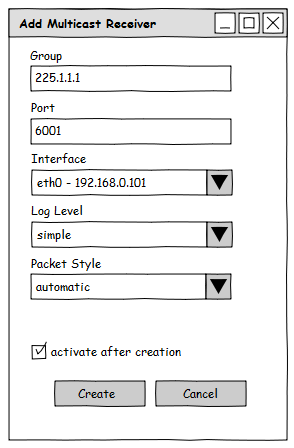
\includegraphics[scale=0.5]{images/gui/addrec.png}
\caption{Hinzufügen eines Empfängers}
\end{figure}
Das Hinzufügen eines neuen Empfängers analog zu oben.

\begin{figure}[H]
\centering
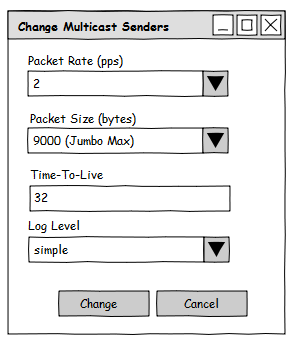
\includegraphics[scale=0.5]{images/gui/changesender.png}
\caption{Ändern eines Senders}
\end{figure}
Beim Umkonfigurieren von Sendern können bei Mehrfachauswahl sinnvolle Parameter
bequem für alle Datenströme auf einmal geändert werden.

\begin{figure}[H]
\centering
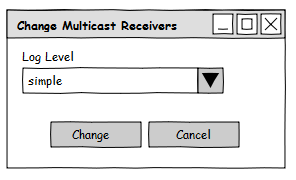
\includegraphics[scale=0.5]{images/gui/changerec.png}
\caption{Ändern eines Empfängers}
\end{figure}
Das Umkonfigurieren von Empfängern analog zu oben.

\begin{figure}[H]
\centering
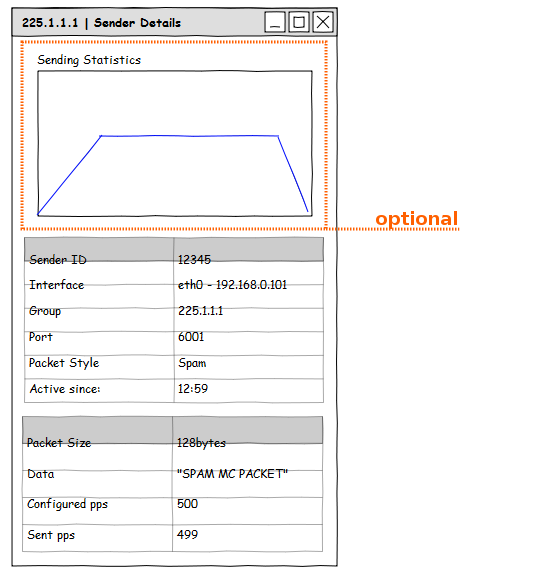
\includegraphics[scale=0.5]{images/gui/detailssender.png}
\caption{Detailansicht eines Senders}
\end{figure}
Benötigt man genauere Informationen zu einem bestimmten Datenstrom, kann man
sich eine detaillierte Sicht anzeigen lassen. In dieser werden alle vorhandenen
Informationen dargestellt. Zu Beachten: Die graphische Darstellung der
Datenströme ist eine optionale Anforderung, ihre Implementierung in Version 1
ist noch nicht sicher.

\begin{figure}[H]
\centering
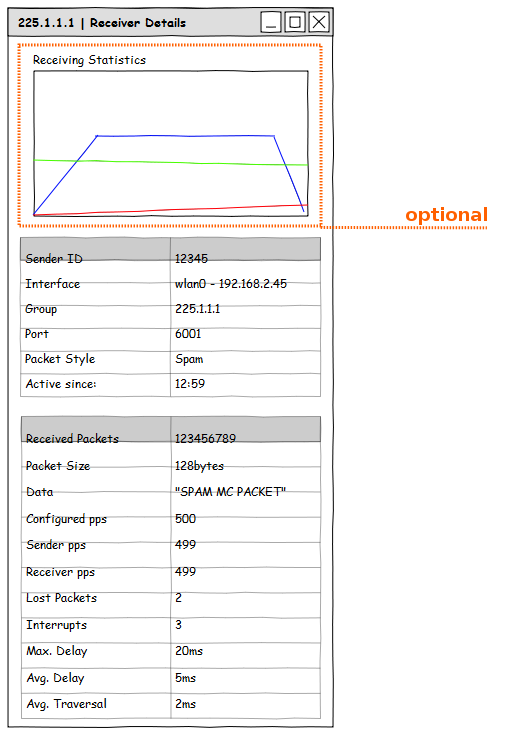
\includegraphics[scale=0.5]{images/gui/detailsrec.png}
\caption{Detailansicht eines Empfängers}
\end{figure}
Detailansicht eines Empfängers analog zu oben.

\begin{figure}[H]
\centering

\includegraphics[scale=0.5]{images/gui/error.png}
\caption{Beispiel für Fehleranzeige}
\end{figure}
Bei falschen Eingaben oder Programmfehlern wird em Nutzer eine einfach
verständliche und eindeutige Fehlermeldung angezeigt.

	
	\chapter{Standard Java Coding Convetions}
	\label{a:code}
	Ab der nächsten Seite bis zum Ende des Dokuemnts finden sie die Standard Java Coding Convetions (1997).
	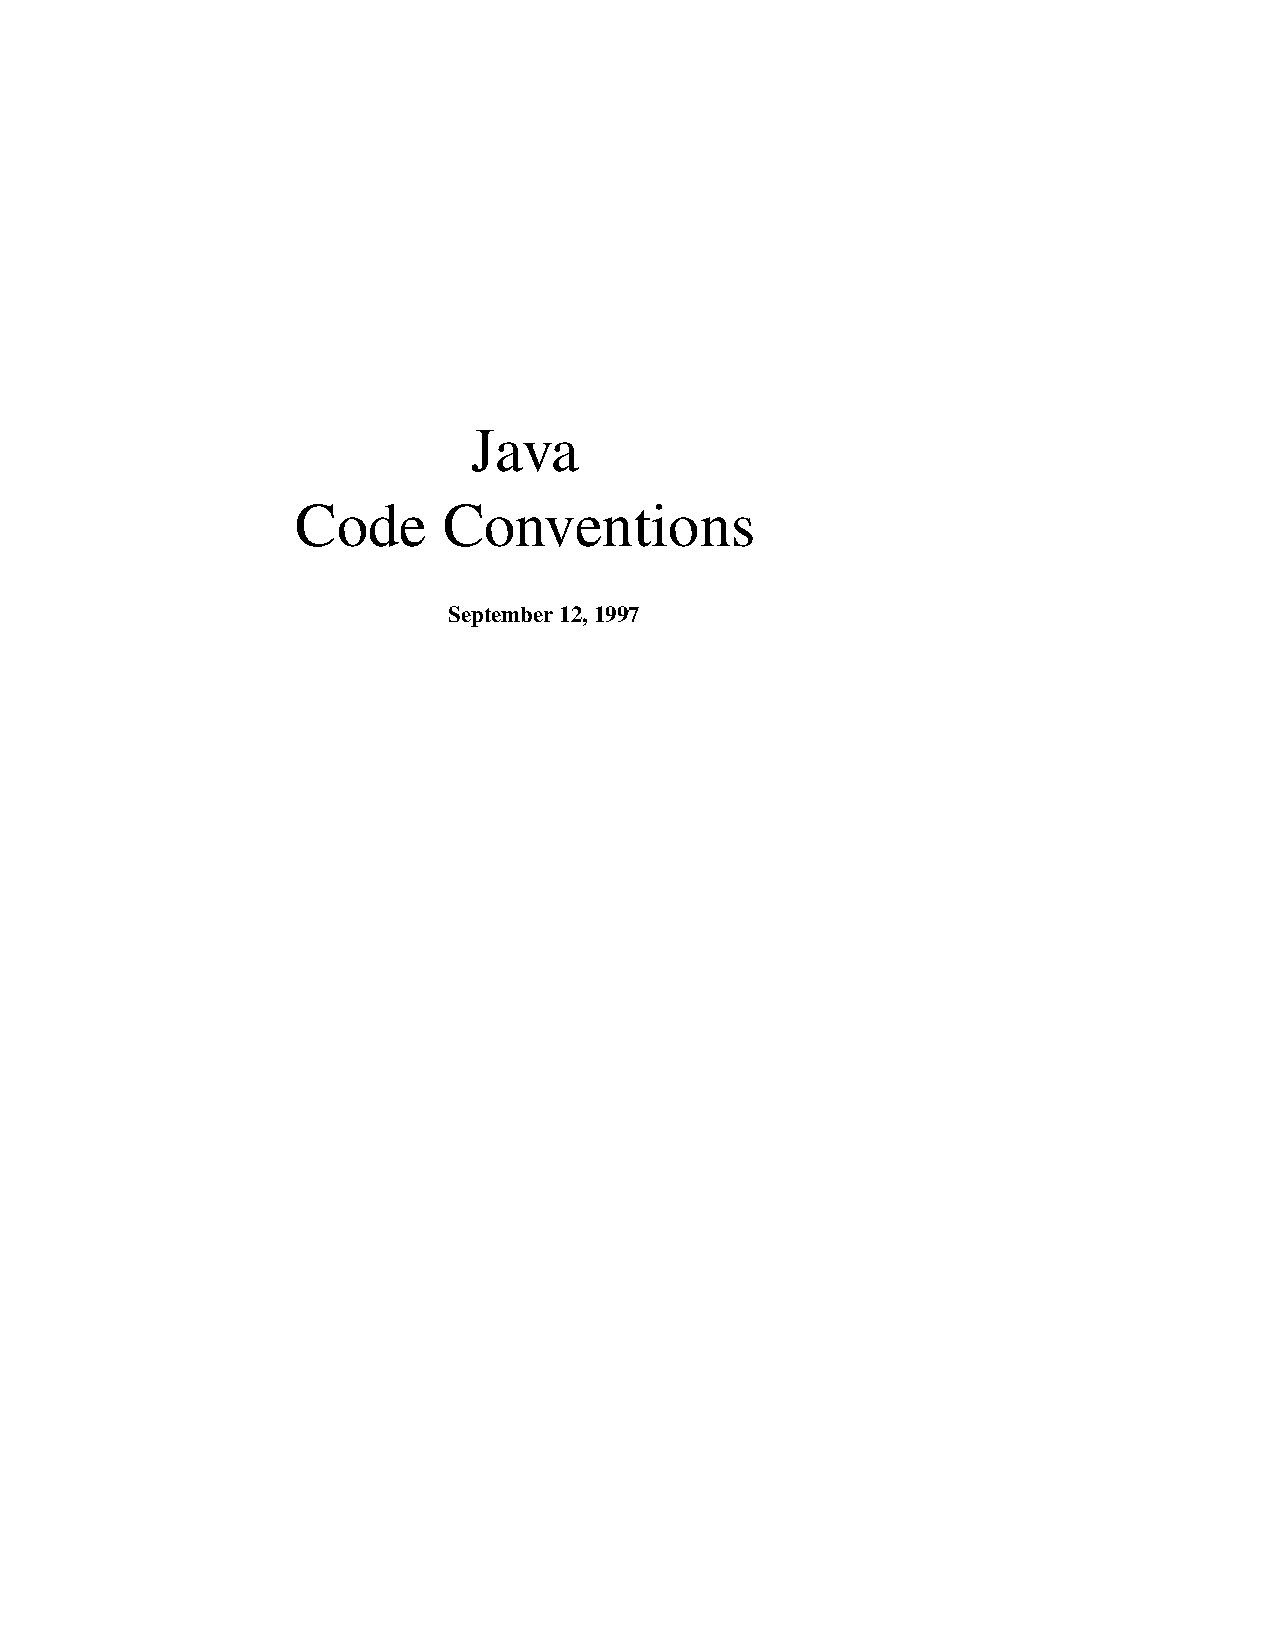
\includepdf[pages=1-23, pagecommand={\thispagestyle{headings}}]{codeconventions-150003.pdf}

	\dots{}
 	\end{appendix}
	%%%%%%%%%%%%%%%%%%%%%%%%%%%%%%%%%%%%%%%%%%%%%%%%%%%%%%%%%%%%%%%%%%%%%%%%%%%%%%%%

	% Anhang
	%\include{./chapter/appendix}
	%%%%%%%%%%%%%%%%%%%%%%%%%%%%%%%%%%%%%%%%%%%%%%%%%%%%%%%%%%%%%%%%%%%%%%%%%%%%%%%%


	% Literaturverzeichnis
	%\nocite*{}
	%\bibliographystyle{gerplain}
	%\bibliography{literatur}
	%%%%%%%%%%%%%%%%%%%%%%%%%%%%%%%%%%%%%%%%%%%%%%%%%%%%%%%%%%%%%%%%%%%%%%%%%%%%%%%%

% Dokumentende
\end{document}